\documentclass[10pt]{article}
\usepackage{graphicx}        % standard LaTeX graphics tool

%-------
%Packages
%-------
%Extra packages
\usepackage{palatino}
\linespread{1.05}         % Palatino needs more leading (space between lines)

%\usepackage{times}
\usepackage[tight,footnotesize]{subfigure}
\usepackage[bottom]{footmisc}% places footnotes at page bottom
\usepackage{url}
\usepackage{color}
\usepackage{array}
\usepackage{colortbl}
\usepackage{multirow}
\usepackage{booktabs}
\usepackage{tabularx}
\usepackage{amssymb}
\usepackage{amsmath}
\usepackage{theorem}
\usepackage{wrapfig}

%\usepackage{mathptmx}       % selects Times Roman as basic font
%\usepackage{helvet}         % selects Helvetica as sans-serif font
%\usepackage{courier}        % selects Courier as typewriter font
%\usepackage{type1cm}        % activate if the above 3 fonts are not available on your system
%\usepackage{makeidx}         % allows index generation
%\usepackage{multicol}        % used for the two-column index
%\usepackage{colortbl}
%\usepackage{rotating}
%\usepackage[geometry]{ifsym}

\newenvironment{packed_itemize}{
\begin{itemize}
  \setlength{\itemsep}{1pt}
  \setlength{\parskip}{0pt}
  \setlength{\parsep}{0pt}
}{\end{itemize}}

\newenvironment{packed_enumerate}{
\begin{enumerate}
  \setlength{\itemsep}{1pt}
  \setlength{\parskip}{0pt}
  \setlength{\parsep}{0pt}
}{\end{enumerate}}


% Labels 
% Equation
%\newcommand{\eref}[1]{Equation~\ref{#1}}
% Section
%\newcommand{\sref}[1]{Section~\ref{#1}}
% Figure
%\newcommand{\figref}[1]{Figure~\ref{#1}}
% Algorithm
%\newcommand{\aref}[1]{Algorithm~\ref{#1}}
\setlength{\headheight}{0.1in}
\setlength{\headsep}{0.2in}
\setlength{\textheight}{8.65in}
\setlength{\textwidth}{6.2in}
\setlength{\topmargin}{-0.2in}
\addtolength{\oddsidemargin}{-0.6in}
\addtolength{\evensidemargin}{-0.6in}

%------------------
%Command redefinition
%------------------
\newcommand{\draftnote}[1]{\marginpar{\tiny\raggedright\textsf{\hspace{0pt}#1}}}
\begin{document}



%\centerline{\Large\bf NRI:  Design and Fabrication of Robot Hands for Dexterous Tasks }
%\section{Summary}

Introduction:

Dexterity is a Grand Challenge goal in robotics today, and is on the critical path to capable robots in almost every domain:  home, work, space, medicine, disaster scenarios...    With advances in rapid prototyping and design optimization, we are well poised for dramatic progress in robot dexterity.   Rapid prototyping technologies are becoming available in every lab.    New robot hands are being designed at an unprecedented pace.

However, we are missing one crucial ingredient:  we do not yet fully understand manipulation.   We have no clear guidelines for creating the robot dexterity that would cause a transformative advance.   The lack of clear design goals is a great barrier to further progress, and we as a field are struggling greatly to create reliable, apparently effortless dexterous behavior.

Our proposal aims to address this gap.   We have observed patterns in human manipulation strategies and actions such that we are able to create Grasp Nets representing families of dexterous behavior.    These Grasp Nets provide the design focus that has been lacking.    Our expertise in grasp and manipulation analysis (PI Pollard) and optimal design, rapid prototyping, and control (PI Coros) make us the perfect team to convert these observations  into robot hands that present previously unseen levels of robust dexterous behavior.

Intellectual Merit:

Our working principles and research questions are that:
(A) On-task compliance reduces actuator requirements.   This is important for dexterous manipulation, because keeping number of actuators low and size of actuators small makes it possible to design lightweight hands with less tendon routing (or other actuator complexity to get them off board of the hand).
(B) Joint limits improve robustness to error and likely make it easier to learn a task.
(C) Working from specific Grasp Nets (such as we observe people to use) focuses design efforts and will make possible the next quantum leap in design for dexterous manipulation.

We will advance the state of the art in:
(1) Creation of Grasp Nets capturing broadening collections of grasping and manipulation capability as observed in human performance.
(2) Design, modeling, and optimization of compliant elements to simplify manipulation task performance.
(3) Analysis of manipulation with joint limits.
(4) Design and optimization of joint limit surfaces to improve robustness of grasping and manipulation actions.
(5) Development of models of error and variation in state of the art manufacturing technologies as they relate to dexterous manipulation.
Together, these contributions will make possible for the first time reliable and broadly varying dexterous behavior from accessible designed prototyping technologies.

Broader Impact:

Having truly dexterous robots will affect many areas of our lives.   If robots can suddenly use their hands in a dexterous manner, they will be able to create nontrivial effects on the world and be capable of rendering competent assistance in manual tasks and applications can improve our quality of life, our health, and our safety.     Educational broader impact includes K-12 outreach efforts.  For example, we have recently brought the discussion of robot hands in to the elementary school classroom.    Evaluation metrics will be available to be part of the continuing efforts to develop grasping and manipulation benchmarks.   Grasp Nets and robot hand designs will be made available so that others can easily access and build upon our results.   The PIs have an excellent track record with mentoring underrepresented students and undergraduates and will continue this trend.



%\newpage

\section{Introduction}

Robot dexterity is critically important for robots working alongside people and for robots working in human spaces.    Robots must be able to manipulate human objects and use tools made for people in order to assist people in performing tasks from mission critical to everyday.   

Unfortunately, despite decades of development of high degree-of-freedom dexterous robot hands since the 80's, dexterous manipulation has remained elusive.  Dexterity is a Grand Challenge goal.   In fact, the 2013 Robotics Roadmap \cite{christensen2009roadmap} states:
\begin{quotation}
{\small \it
Robot arms and hands will eventually out-perform human hands. This is already true in terms of speed and strength. However, human hands still out-perform their robotic counterparts in tasks requiring dexterous manipulation. This is due to gaps in key technology areas, especially perception, robust high fidelity sensing, and planning and control. The roadmap for human-like dexterous manipulation consists of the following milestones:
\begin{itemize}
	\item 5 years: Low-complexity hands with small numbers of independent joints will be capable of robust whole-hand grasp acquisition.
	\item 10 years: Medium-complexity hands with ten or more independent joints and novel mechanisms and actuators will be capable of whole-hand grasp acquisition and limited dexterous manipulation.
	\item 15 years: High-complexity hands with tactile array densities, approaching that of humans and with superior dynamic performance, will be capable of robust whole-hand grasp acquisition and dexterous manipulation of objects found in manufacturing environments used by human workers.
\end{itemize}}
\end{quotation}
In this set of milestones, dexterous manipulation is not mentioned for the 5 year mark.   Dexterity is expected in limited form at 10 years, and approaching human levels in 15 years.

{\it We propose to enable dexterity at the 5 year mark through task directed design with emphasis on the role of joint limits and compliance.}

There are many very excellent research groups working on the critical areas of sensing, planning, and control.   Our approach is orthogonal and complementary to these efforts.    We aim to reduce the load on sensing, planning and control by designing the mechanism to be as favorable to the intended task set as possible by developing new analysis and design tools for crafting the robot hand to make dexterous manipulation easier from the start.

Our approach centers around several elements:  (1) "Grasp Net" benchmarks to explore manipulation at its full complexity, (2) Mechanism design focused on specific tasks that are well known (i.e., the Grasp Nets), (3) Strategic Placement of Actuators, Joint Limits, and Compliance, and (4) Strategic consideration of Sensing.

\smallskip\noindent
{\bf (1) "Grasp Net" benchmarks to explore manipulation at its full complexity.}   To tackle dexterous manipulation head-on, we must consider grasping and manipulation in its full complexity.   We take inspiration from human dexterity.   Full scale humanlike dexterous manipulation may appear enormously complex.   However,  we have observed a relatively small number of grasping tasks and manipulations that are used over and over, with common actions linked to one another, forming what we call Grasp Nets.   These Grasp Nets give us a way to proceed without oversimplifying.  We propose to create Grasp Net benchmarks to cover expanding portions of the dexterous manipulation space.   In tandem, we will develop evaluation procedures that test ability of a mechanism to accomplish Grasp Net tasks in the presence of uncertainty.   One project goal is to create and debug these tests to contribute them to the Roadmap to Progress Measurement Science in Robot Dexterity and Manipulation \cite{falco2014roadmap} where evaluation metrics for dexterous manipulation are needed.

\smallskip\noindent	
{\bf (2) Mechanism design focused on specific tasks that are well known (i.e., the Grasp Nets).}   Mechanisms will be designed specifically to accomplish grasps and manipulations within the Grasp Nets, manufactured, and evaluated on the Grasp Net benchmarks in an iterative process.
Even the initial Grasp Nets will include families of objects for generality.   They will reflect real-world manipulations and assume considerable uncertainties and variation.   But they will be concrete lists of benchmarks that the hand must accomplish, facilitating rapid evaluation and design exploration.   Our goal is to pursue generality while rooting our evaluation of possible hand designs solidly in useful tasks in the real world.

\smallskip\noindent
{\bf (3) Strategic Placement of Actuators, Joint Limits, and Compliance.}  We believe that the keys to robustness of hand designs will be selection and placement of a small number of actuators, generous use of joint limits, and strategic use of built-in compliance.    We will explore a variety of actuator designs and mechanisms.   We will develop new tools to analyze manipulation capabilities in the presence of are scale compliance and joint limit surfaces.    Theoretical developments and models will be validated and improved with experimental data collected from many design iterations, component testing, and system testing. 

\smallskip\noindent
{\bf (4) Strategic consideration of Sensing.}    Sensor design will be considered in later stages of the project with the point of view of what type of sensor could most improve performance of the mechanism on its intended tasks (e.g., increase generality or robustness and/or eliminate catastrophic failure).  Primarily reflex and error correcting behaviors will be considered, e.g., response to slipping of the grip, total loss of contact, or stopping of expected motion.   It is encouraging that in our human subjects studies we observe frequent failures such as collisions prior to reaching the intended destination, which are resolved with characteristic corrections.   Our first line of attack will be to enable similar behavior.
	
PI Pollard brings decades of experience in grasping and manipulation analysis and experience working with various robotic hands and systems.   PI Coros brings experience in optimal design of creative, complex mechanisms to accomplish user specified tasks, as well as 10 years of experience in control algorithms for complex tasks.     This combination of skills is critical for designing and creating robot hands with the capability and skills to grasp and manipulate robustly in complex, real-world scenarios where humans and robots live and work together.

       % Nancy

\section{A Simple Example}

In this section, we work out a simple example for purposes of illustrating our proposed approach.

\begin{figure}
\begin{center}
%{\includegraphics[width=6in]{./images/wrenchPickup.png}}
\vspace*{2in}
\end{center}
\caption[]{This trivial Grasp Net nonetheless captures two important grasps and a dexterous motion to move between them.}
\label{SimpleGraspNet}
\end{figure}

Consider the trivial Grasp Net show in Figure~\ref{SimpleGraspNet}.     This figure shows two grasps.   Grasp A is a pinch grasp, typical for lifting objects from a surface, placing them down, performing certain dexterous actions such as using tweezers, and as a staging point for moving to other grasps (e.g., consider lifting a wrench and then maneuvering it to enclose it within the palm).    Forces in the pinch grasp oppose one another along the local y-axis.   Objects may be of varying width, and grasp force may vary, creating a family of pinch grasps we would like the robot to be able to achieve.

Grasp B is a lateral grasp, often called the key pinch grasp, useful for comfortably and securely holding objects, for certain assembly operations (e.g., put a key or a card into a slot), and for offering an object to a person (or another robot).   Forces for the lateral grasp in this example oppose one another along the x-axis.  We consider the same object set, but rotated 90 degrees.   Greater forces may be desired for this grasp.   As with all grasps, we specify an exact set of relative contact locations and forces that defines our grasp.

Manipulation 1 is used to move between the two grasps.   In this case we can imagine the "thumb" pivoting around the "index finger," although in our final design, the motion may be generated by either or both fingers.    The variation in object widths creates a family of curves describing motion of the thumb relative to the finger.   The object is specified to slide on the finger so that the thumb contact remains nearly constant.

Forces in this example do little more than guarantee that the object remains secured while performing the manipulation.   The manipulation is assumed to be quasistatic.

A successful design must be able to move all of the benchmark objects from Grasp A to Grasp B using Manipulation 1.

Suppose that a mechanism designer has specified the following design constraints and suggestions:
\begin{itemize}
   \item Actuators apply unidirectional linear force in the finger coordinate frame (e.g., tendons acting through the finger center of mass).
   \item Fingers can be made to be passively compliant using a linear stiffness model.  [STELIAN GIVE ME A BETTER STIFFNESS MODEL.]
   \item At any time instant, at least one force must be active.
   \item Force directions during static grasping may be good directions in which to actuate a finger.
   \item Force directions during static grasping may be good directions in which to craft joint limits.
\end{itemize}

Suppose further that the designer's goals, in order of priority, are:
\begin{enumerate}
	\item Grasp and manipulate all benchmark objects as specified in the Grasp Net.
	\item Minimize the total number of actuators.
	\item Minimize the number of actuators per finger.
	\item Minimize the sum of forces that are actively applied (i.e., joint limits and passive forces due to compliance are "free")
\end{enumerate}

For Goal 2, a test of rank on relative positions will determine that the minimum number of actuators is two.

For Goal 3, a tree search will find we can split these actuators between the fingers, so that each has one degree of freedom.

Now, we are left with 8 choices, as the thumb can be actuated in any of the four coordinate axis directions, and in each case there would be two choices of direction in which to actuate the index finger (specifically [x, y], [x, -y], [-x, y], [-x, -y], [y, x], [y, -x], [-y, x], [-y, -x]).

Figure~\ref{SimpleExampleResults} shows one final solution, where the thumb is actuated along the negative x-axis and the index finger is actuated along the negative y-axis.   This is perhaps the most humanlike example and most resembles hands which actuate the grasping forces and use return springs to bring the fingers back to a fully open pose.   

[SAY SOMETHING ABOUT JOINT LIMITS AND SPRINGS.]

[EXPLORATION:   (1) THUMB GETS Y .. ANY DIFFERENCE?   (2) VALUE OF 4 ACTUATORS?]

We can compare work done in the various cases, including without compliance.

\begin{figure}
\begin{center}
%{\includegraphics[width=6in]{./images/wrenchPickup.png}}
\vspace*{2in}
\end{center}
\caption[]{Final solution.}
\label{SimpleExampleResults}
\end{figure}


  % Nancy

\section{Dexterous Manipulation Analysis with Joint Limits and Compliance}

\begin{figure}
\begin{center}
%{\includegraphics[width=6in]{./images/wrenchPickup.png}}
\vspace*{2in}
\end{center}
\caption[]{Several designs with the goal of robust pushing.}
\label{PushExample}
\end{figure}

\begin{figure}
\begin{center}
\begin{tabular}{l|c|c|c|c|c|c|c|}
Design & x0 & y0 & kx & ky & cost &	actuated x range &	actuated y range \\ \hline
(A) 4 tendons, no compliance&	-&	-&	-&	-&	1600	&(-4, 0)	&(-4, 0)\\
(B) 4 tendons, compliance	&-1.887	&-2.58	&0.54&	0.43&	{\bf 107.65} &	(-1.36, 1.02)	&(-1.61, 1.11) \\
(C) 2 tendons, spring open&	7	&7	&min	&min	&1600	&(-4, 0)	&(-4, 0)\\
(D) 2 tendons, spring closed&	-5.883&	-4.998&	0.45&	0.5	& {\bf 445.3}  &	(0, 2.65)&	(0, 2.49)\\
\end{tabular}
\end{center}
\caption{Optimal parameters, cost, and actuator range for several mechanism designs to perform Grasp A, Grasp B, and Manipulation 1.}
\label{ComplianceAnalysis}
\end{figure}

From the simple example of Figures~\ref{SimpleGraspNet} and \ref{SimpleExampleResults}, we can show two things:  (1) Careful design of compliance can reduce the number of actuators and actuator load, and (2) Joint limits can be important for robust performance of a manipulation and perhaps also contribute to making the manipulation easy to learn.   Furthermore, using a different example shown in Figure~\ref{PushExample}, we show a little of how (3) we can expand our analysis tools to consider design with joint limits.  Finally, in the next section, we discuss optimization of complex mechanisms to accomplish Grasp Net tasks.

\smallskip\noindent
{\bf (1) Compliance matters.}  Table~\ref{ComplianceAnalysis} shows results for four tendon driven designs, which were optimized to perform Grasp A, Grasp B, and Manipulation 1 for 4 objects of varying widths.   Quasistatic analysis was performed for each design, with actuators for the thumb moving in the X direction, and actuators for the finger moving in the Y direction.  The quasi static analysis ensured that forces required for Grasp A, Grasp B, and Manipulation 1 could be generated by the mechanism.   Each design was optimized using CMA \cite{hansen2006cma} to require the minimum total actuation force, expressed as squared actuated forces summed over objects, actuators, and time samples.    Where compliance was considered, linear springs were assumed, and the algorithm optimized for spring zero point and stiffness.   Optimal parameters, cost, and range of actuated forces are shown in the Figure.

Design (A) contains 4 tendons, which give active control in both the negative and positive X directions for the thumb and the negative and positive Y directions for the finger.   This design considers no passive compliance.   Design (B) contains the same 4 tendons, but it also includes linear springs.   Note that the cost of forces provided by the actuators is less than 7 percent that of Design (A).    Design (C) has only two tendons, which are used as elastic return springs, opening the hand.    The presence of the spring elements reduces the total number of actuators, but does not reduce the cost of the design.    Design (D) also has two tendons, which are employed to open the fingers.    Here, the total cost is 28 percent of that of Design (A), and has been achieved with half the number of actuators.    Clearly, compliance matters to reduce the total number of actuators and to reduced actively applied forces for actions in the Grasp Net.

\begin{figure}
\begin{center}
\begin{tabular}{l|c|c|c|c|c|}
Test Case & \multicolumn{5}{c}{Errors at Gaussian perturbation (radians)}  \\
                & None & 0.1  & 0.2  & 0.3  &  0.4  \\ \hline 
(A) Joint limits, learn with perfect mechanism &	{\bf 0.01} & 0.90 & 1.63 &	2.32 & 3.61 \\
(B) Joint limits, learn with perturbation	&  {\bf 0.04}	& {\bf 0.05}	& {\bf 0.08} &	{\bf 0.21} &	1.42 \\
(C) No joint limits, learn with perfect mechanism &	{\bf 0.01}	&	1.05&	2.13	& 2.84  &	4.06 \\
(D) No joint limits, learn with perturbation &	{\bf 0.03}	& {\bf 0.06} 	&1.43	&4.38	&5.75 \\
\end{tabular}
\end{center}
\caption{This exploration shows the value of joint limits.   Mean error of an optimized manipulation is shown as perturbations to the perfect mechanism grow in magnitude.    Standard deviation is in parentheses.  The test having both joint limits and optimized while seeing small perturbations is able to handle perturbations three time the size of any other situation tested.}
\label{JointLimitAnalysis}
\end{figure}

\smallskip\noindent
{\bf (2) Joint Limits matter.}   We observe that joint limits are not avoided in human motion.   In contrast, in the human system, joint limits and singularities are often exploited.    The limit at our knee that facilitates straight leg walking is a well known example, but there are many examples in grasping and manipulation as well.  In a lateral grasp (which motivated Grasp B), the moderately flexed fingers can passively support large lateral forces, even though the force that cana be actively generated by forces in that grasp is small, coming from small intrinsic muscles in the hand, such as the interossei \cite{brand1999clinical}.   These large forces are available because the fingers are operating near their joint limits in this direction.   As another example, large forces can be transmitted through our palm all the way up to our strong shoulder muscles, or even through to the ground in some cases.   Pressing hard with a fingertip will also exploit joint limits.

Here, we show one simple example that joint limits can make a practical difference.   In this set of tests, we explored the ability to learn robust open loop control for Manipulation 1.    Motor velocities for the thumb and finger were represented as linear functions of time, with three velocity control points per finger, resulting in a search space of six parameters.   CMA was used to optimize these parameters.    Box2D was used to simulate the manipulation for any given parameter set.   The cost at the end of each simulation was the difference between the final object configuration and that desired for Grasp B.     Once an optimal open loop motion had been identified by the optimizer, it was evaluated on a series of 5 tests, each involving 100 simulations having perturbations in the direction of motion of the finger.    Finger motion direction was perturbed about its intended direction using a normal distribution with standard deviation of 0, 0.1, 0.2, 0.3, and 0.4 radians.    The motivation for this choice is that in a more complex hand, it is often difficult to know exactly where the fingers are relative to one another, and this variation can affect ability to manipulate robustly.   When a test used joint limits, the limits for the thumb were placed in the X direction, both at the thumb's origin in Grasp A and at a wide open position that gave clearance twice the width of the largest object.   Joint limits for the finger, when used, were placed in the Y direction, both at its destination in Grasp B and in a wide open position that gave clearance twice the width of the largest object.

Four cases were considered.   In Case (A), joint limits were included, and the manipulation action was optimized assuming a perfect mechanism.   Case (B) is similar to Case (A), but included random perturbations during the learning phase, having a standard deviation of 0.2 radians.    Cases (C) and (D) are variations where joint limits are not included.   Table~\ref{JointLimitAnalysis} shows the results.   Empirically, results with error less than 0.5 in our scale produced consistently good results.   These results show that when a task is learned assuming a perfect mechanism, the effect of joint limits is not clear.    However, when the learning process has the opportunity to see the perturbations, the optimizer learns to use the joint limits to create compensating strategies.    Case (B), including both joint limits and learning with perturbations, is able to handle three times the amount of disturbance of any other case.      Based on qualitative observation only, the cases having joint limits also appeared to present easier learning problems.

\smallskip\noindent
{\bf (3) We must expand our analysis tools to consider design with joint limits.}     Consider now the example in Figure~\ref{PushExample} A.     The goal here is to push into a surface, holding the object in more or less the given grasp.   There will be variation in the task, as the object may contact the surface at different points and with different surface contact normals, resulting in varying force directions and moment about the object center of mass.    Each finger has one tendon to actuate it, and the directions of actuation are shown.    We assume the two fingers on the sides have considerable compliance in the horizontal direction.   Actuating these fingers does not help either, as this will only cause the fingers to slide along the object surface.    With the design as shown in Figure~\ref{PushExample} A, the grasp will only be able to apply a very small range of task related forces to the object.

We can examine the force balance equations for this situation.   Because the fingers are very compliant, forces on the fingers must be balanced to prevent them from moving:
\begin{equation}
    f_{s, i} +     f_{a, i} +     f_{JL, i} +     f_{c, i} = 0
\end{equation}
Parameter $f_{s, i}$ is the spring force, with a component due to deviation of the initial contact location $c_i$ from rest position $c_{i, 0}$ and a second component due to object motion that results from unequalized forces $\Delta X_o$, which is intended to be small for a good grasp.   Matrix $K_i$ encodes stiffnesses and $G_i$ is the grasp matrix for finger i.
\begin{equation}
 f_{s, i} = -K_i ( c_i - c_{i, 0}) - K_i G^T_i \Delta X_o
\end{equation}
Parameter $f_{a, i} = D_i P_i A_i$ is force generated by the actuators as in \cite{Li:graspDB07}, and is expressed using activation levels $A_i$, such that $0 \leq a_i \leq 1$, diagonal matrix $P_i$ of maximum actuator forces, and matrix $D_i$ of actuator directions.
Parameter $f_{JL, i}$ is the novel component compared to other treatments that consider grasp quality measures for compliant systems (e.g., \cite{lin2000stiffness}), and can be expressed for a frictionless joint limit surface as:
\begin{equation}
	f_{JL, i} = -k_{JL} N_i S_i N^T_i      G^T_i \Delta X_o
\end{equation}
with joint limit normal matrix $N_i$ and (large) stiffness experienced at the limit of $k_{JL}$.    Note the selector matrix $S_i$ which indicates which joint limits relevant to finger i are currently engaged by some external or active force.
Parameter $f_{c, i}$ is the contact force, which must be within the friction cone at the contact and contributes to balancing a desired external wrench $W_{ext}$ due to the pushing contact with the ground in this case:
\begin{equation}
  - \sum_i G_i f_{c, i} = W_{ext}
\end{equation}
For a given value of selector matrices $S_i$, we can solve the resulting linear system for actuator forces $A$ and object motion $\Delta X_o$.    In a valid solution, $\Delta X_o$ must be consistent with $S_i$ such that the object motion pushes the object into the limit to engage it.   The system as a whole can be resolved through pivoting or other discrete search techniques.

This setup can also be used for design.   As mentioned above, the side fingers in Figure~\ref{PushExample} A are not at all helpful for accomplishing the task.  A search for optimal joint limits may result in Figure~\ref{PushExample} B, which is similar to using two fingers laterally as guides while pushing with a middle finger.   Here, the range of task forces that can be applied is considerably greater.     Torques due to ground contact forces at the object base engage one of the joint limits, allowing a force balance to be created.

A third option, shown in Figure~\ref{PushExample} C, is to add an additional actuator that can actively engage the joint limit opposite to it.   The result is a very strong grasp, reminiscent of human power lateral grasps, which can easily provide the task forces and many more.   As a side benefit, the two previously useless actuators can now contribute to the task, sharing the load with the actuator of the top finger.

In each case, the force balance equation as shown here, along with a straightforward linear optimization to compute the set of task forces that can be equalized (following our own work \cite{Li:graspDB07}), have made it possible to evaluate the effect of any new design element on the push grasp.

Extension to complex and redundant mechanisms is more complex, and is the subject of future research.

    % Nancy

\section{Dexterous Hand Design / Optimization}
  \label{secHandDesign}

\newcommand{\bA}{\mathbf{A}}
\newcommand{\bB}{\mathbf{B}}
\newcommand{\bC}{\mathbf{C}}
\newcommand{\bD}{\mathbf{D}}
\newcommand{\bE}{\mathbf{E}}
\newcommand{\bF}{\mathbf{F}}
\newcommand{\bG}{\mathbf{G}}
\newcommand{\bH}{\mathbf{H}}
\newcommand{\bI}{\mathbf{I}}
\newcommand{\bJ}{\mathbf{J}}
\newcommand{\bK}{\mathbf{K}}
\newcommand{\bM}{\mathbf{M}}
\newcommand{\bR}{\mathbf{R}}
\newcommand{\bU}{\mathbf{U}}
\newcommand{\ba}{\mathbf{a}}
\newcommand{\bb}{\mathbf{b}}
\newcommand{\bc}{\mathbf{c}}
\newcommand{\bd}{\mathbf{d}}
\newcommand{\be}{\mathbf{e}}
\newcommand{\bff}{\mathbf{f}}
\newcommand{\bg}{\mathbf{g}}
\newcommand{\bk}{\mathbf{k}}
\newcommand{\bm}{\mathbf{m}}
\newcommand{\bn}{\mathbf{n}}
\newcommand{\bp}{\mathbf{p}}
\newcommand{\bs}{\mathbf{s}}
\newcommand{\bt}{\mathbf{t}}
\newcommand{\bu}{\mathbf{u}}
\newcommand{\bv}{\mathbf{v}}
\newcommand{\bx}{\mathbf{x}}
\newcommand{\bl}{\mathbf{l}}
\newcommand{\bq}{\mathbf{q}}
\newcommand{\bw}{\vec{w}}
\newcommand{\bX}{\mathbf{X}}
\newcommand{\bS}{\mathbf{S}}
\newcommand{\bj}{\mathbf{j}}
\newcommand{\bT}{\mathbf{T}}
\newcommand{\bP}{\mathbf{P}}

\newcommand{\bbx}{\bar{\bx}}

%relevant work to discuss: http://biorobotics.harvard.edu/robotic_hand_optimization.html
%http://bbdl.usc.edu/Papers/2013_IJRR_Inouye_Anthropomorphic_Hand.pdf

Recent work has shown that carefully engineered mechanical designs can prove crucial in improving the versatility of robotic manipulators for static grasping tasks~\cite{Ciocarlie:2014:VGV:2674203.2674213}. The aim of our work is to generalize this concept in order to revolutionize dexterous manipulation in the same way. We therefore propose mathematical models and algorithmic approaches to co-design mechanical structures and control policies for robotic manipulation tasks. Our hypothesis is that by complementing each other and working in unison, control policies can be significantly simpler, and appropriate mechanical features -- joint stops, compliance, etc. -- can passively improve the robustness of the manipulation tasks while reducing sensing and actuation requirements. 

\subsection{Bottom-up design}

The design process will begin with a specific family of tasks (i.e., a Grasp Net). As described in Section~\ref{secLimitAnalysis}, features such as compliance of passive structures or joint limits can be computed through numerical optimization. Our goal is to automatically translate these optimized features into mechanical structures that can be 3D printed. As a first step, we will investigate bottom-up approaches. For the physical prototype of the 1 degree-of-freedom manipulator shown in Figure~\ref{SimpleExampleResults}, for example, we used a script to generate 3d printable geometry using constructive solid modeling. After fabrication, we used rubber bands to approximately match the optimized compliance of the passive features. The resulting mechanical setup was actuated manually. We view this first result as very encouraging because, with no sensing and very crude actuation, the simple robotic hand was able to reliably and repeatedly perform the manipulation task it was designed for.

Our future investigations will formalize the process we used to design and fabricate our first robotic
\begin{wrapfigure}{hR}{0.25\linewidth}
\vspace{-4mm}
\includegraphics[width=1.0\linewidth]{figs/bendy}
\vspace{-7mm}
\end{wrapfigure}hand. We will begin by building upon the mechanism design work led by PI Coros~\cite{Coros2013,Bacher2015} to automate the synthesis and optimization of assemblies based on trajectories of contact points. We will then extend these models to appropriately control the compliance of the mechanical structures. As illustrated in the inset figure, 3D printing is capable of fabricating objects with complex geometric features, which, in turn, allows the compliance of manufactured parts to be modulated. PI Coros has already started to develop computational methods to explore the relationship between geometric shape, material parameters and deformation behavior~\cite{Skouras2013,Jesus2015}. Briefly, we will model mechanical structures using a Finite Element Method (FEM) approach, where volumetric structures are discretized into a set of elementary shapes (e.g. tetrahedrons). Through a constitutive model, the deformations of the elementary shapes are mapped to elastic energy by integrating over the domain of each element. The global deformation energy $W$ is obtained by summing up elemental contributions, and internal forces are computed as $\textbf{f}_{int} = -\frac{\partial W}{\partial \bx}$, where $\bx$ is an array concatenating the vertex coordinates for each element. Quasi-static configurations for the mechanical structures under load can be obtained by finding the deformed configuration $\bx$ that leads to force equilibrium. Our mathematical models predict how these quasi-static configurations change with the shape of the mechanical parts and their material parameters~\cite{Skouras2013}. We will leverage these models to optimize the internal forces generated when mechanical parts deform as the robot hand performs manipulation tasks. To increase the range of materials that can be used, we will experiment with both 3D printing and laser cutting technologies to manufacture the mechanical components.

\begin{figure}
\begin{center}
{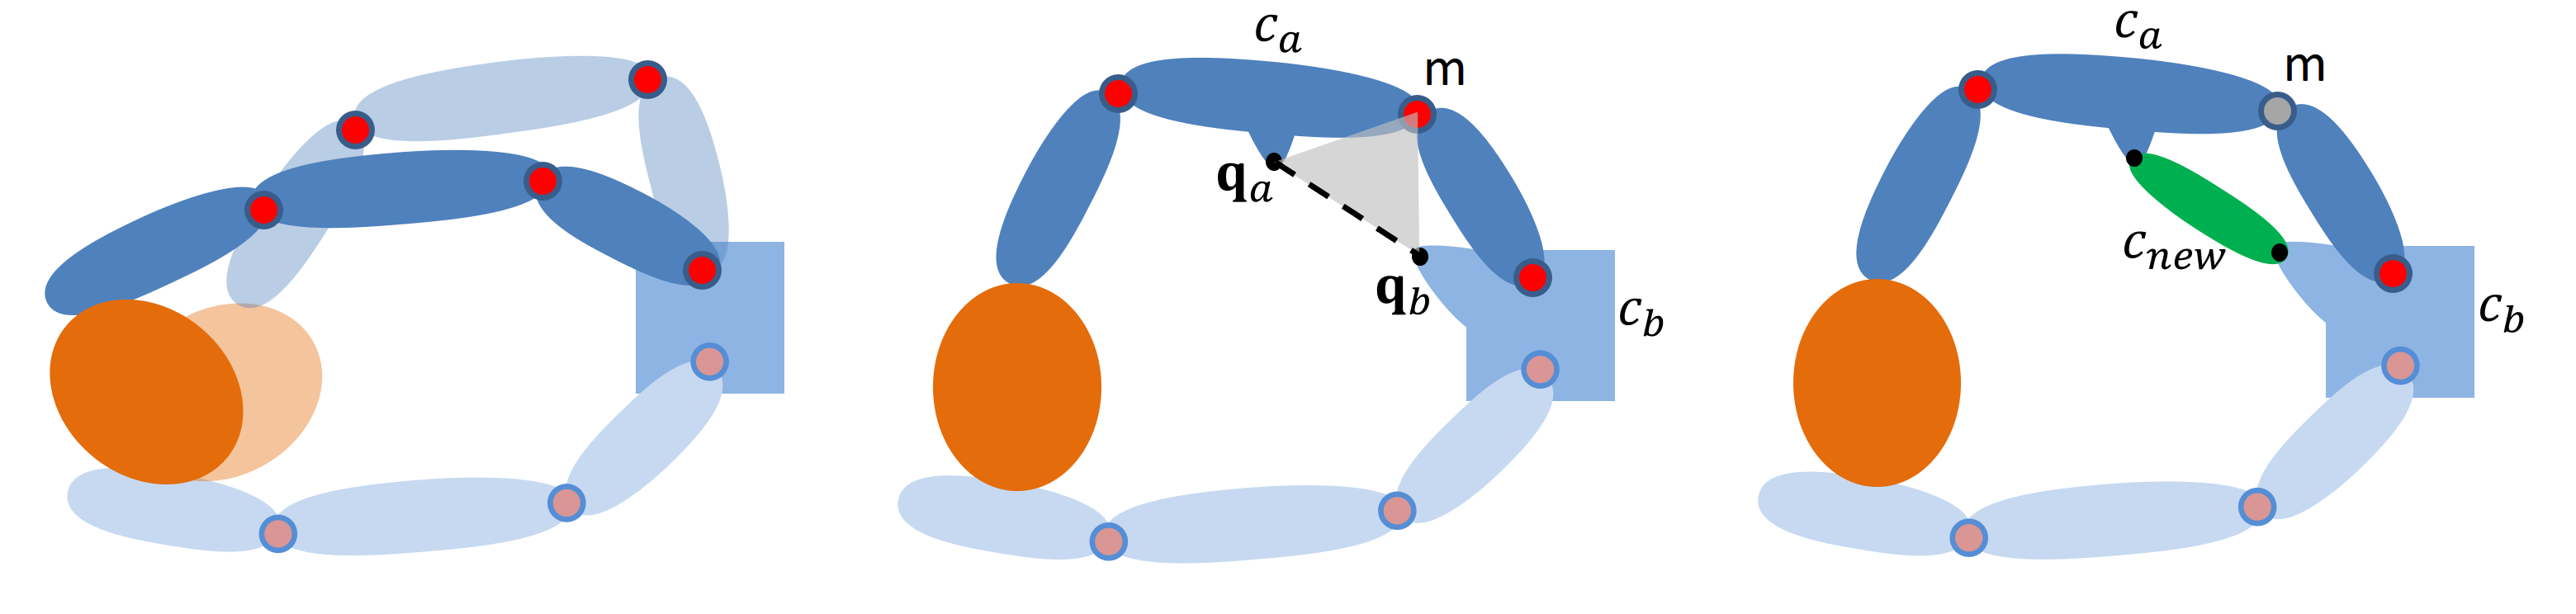
\includegraphics[width=6in]{./figs/handDesign.png}}
\end{center}
\vspace*{-0.2in}
\caption[]{(Left) A conceptual, fully actuated hand design performing a dexterous manipulation task. Active motors are highlighted in red. (Middle) Given two components $c_a$ and $c_b$, we seek a pair of points $\bq_a$ and $\bq_b$ such that the distance between them varies least throughout the motion. To avoid singularities, the area of the highlighted triangle must remain positive throughout the entire motion. (Right) The hand design is simplified by removing motor $m$ and introducing a new passive link $c_{new}$.}
\label{handMechanismDesign}
\end{figure}

\subsection{Top-down design}

While bottom-up approaches aim to create a hand design from scratch, we will also investigate top-down approaches. The strategy here will be to begin with a conceptual design of a highly actuated robot hand design. For example, if a dexterous manipulation task was described through motion capture data, then the initial design would be given by an actuated articulated structure that matches the kinematics of the performer's hand. The underlying assumption is that, with perfect state knowledge and optimal controllers, this robot hand would be able to perform the desired dexterous manipulation tasks. Through an iterative process, the mathematical models we will develop will be used to replace active degrees of freedom with appropriate passive mechanical structures such that a balance between adaptability and simplicity is achieved. 

Figure~\ref{handMechanismDesign} illustrates a conceptual, fully actuated robot hand consisting of rigid links connected to virtual actuators that control their motions. In principle, physical actuators could be used to directly replace their virtual counterparts when fabricating this robot hand. However, this would come at an increased cost, a more complex mechanical design setup, and it would require sophisticated control policies to coordinate all the actuators. As an alternative, we propose an automated design process that iteratively replaces virtual actuators with new rigid or compliant links that appropriately couple the motion of different parts of the hand mechanism. The attachment locations, length and material properties of the new mechanical components will be optimized such that changes to the functionality of the input hand design are minimized. 

The starting point for our investigations is a method recently developed by PI Coros and his colleagues. This method is used to design complex linkage structures that generate a desired motion trajectory~\cite{Thomaszewski14CDL}. The concept behind this method, which we will extend as part of our proposal, is based on a simple observation. Removing a motor and adding a new rigid link preserves the invariant that there are always as many constraints as degrees of freedom in the hand's mechanism: eliminating a motor removes one constraint, adding the (planar) link introduces three degrees of freedom, and two pin joints used to connect the new link to the existing structure result in four additional constraints. The motion of each mechanical component is thus either directly driven by a motor, or is mechanically coupled to that of other components.

To determine which motor should be replaced, and how to optimally insert a new mechanical component, we developed a mathematical model based on the following observation: if the distance $d$ between two points on a pair of existing components does not change as the hand performs a manipulation task, then these components can be connected through pin joints to a new rigid link of length $d$. Although the resulting mechanism would technically be over-constrained, the new link and its pin joints would be completely redundant. Removing a motor along the kinematic chain between the two components would resolve this redundancy while perfectly preserving the original motion. In general, there are no guarantees that such pairs of points always exist. Therefore, given two components, $c_a$ and $c_b$, we seek to find a pair of points $\bq_a$ and $\bq_b$ whose world-space distance varies least throughout the motion. The mean squared world-space distance between these two points is given by $l_{ab}=\frac{1}{n_s}\sum_i^{n_s}||\bq_a(t_i)-\bq_b(t_i)||^2$, where $n_s$ is a number of discrete time samples that span the entire motion, and the variance of this quantity is $ E_\mathrm{variance}=\frac{1}{n_s}\sum_i^{n_s}(||\bq_a(t_i)-\bq_b(t_i)||^2-l_{ab})^2$. When searching for the pair of points that minimize this variance term, it is critical that singular configurations are avoided at all times. As illustrated in Figure~\ref{handMechanismDesign}, when the selected motor ($m$) is removed, the new link ($c_{new}$) becomes responsible for driving the motion of component $c_a$ by direct coupling to component $c_b$. To ensure that the effective moment arm remains sufficiently large at all times, the area of the shaded triangle needs to always remain a safe distance away from zero. This can be accomplished through a log barrier term $E_\mathrm{area} = -\log\sum_i^{n_s}\text{area}\left(\bq_b(t_i),\bm(t_i),\bq_a(t_i)\right)^2$, where $\bm(t_i)$ denotes the world-space position for the motor $m$.

Given two components $c_a$ and $c_b$, which are selected in an outer loop, our mathematical model minimizes a weighted combination of the terms $E_\mathrm{variance}$ and $E_\mathrm{area}$. With gradients and hessians for these objectives readily available, a Newton-Raphson scheme efficiently solves the resulting optimization problem. Once points $\bq_a$ and $\bq_b$ are found, they define a candidate rigid link to be added to the hand mechanism. Our design system then individually removes each motor on the kinematic chain between $c_a$ and $c_b$ and further optimizes the motion of the resulting assembly using our recently developed method~\cite{Bacher2015}. Importantly, this optimization step not only adapts the kinematic parameters of the design, but also the actuator signals that control the motion of the hand mechanism. As a measure of the success of each potential replacement operation, we evaluate the difference in motion between the initial hand design and the optimized mechanism with fewer active degrees of freedom. If the resulting mechanisms deviate too much from the hand's initial motion, a new set of components will be selected and the process repeats. Otherwise, the replacement operation is finalized.

To improve the reliability of the designs generated with our mathematical models, we will develop additional optimization objectives based on the linear robustness analysis introduced by PI Pollard~\cite{Pollard:WAFR02,pollard2004closure,pollard20045}. Further, as described in the previous subsection, we will improve their adaptability by optimizing the compliance of the mechanical links introduced to replace active degrees of freedom. This significant extension will allow the simplified robot hands we design to not only duplicate motion trajectories, but also the contact forces required to manipulate objects.
% This initiative will build on recent methods developed by PI Coros to optimize volumetric~\cite{Skouras2013} and rod-based~\cite{Jesus2015} mechanical structures. Leveraging multi-material 3D Printing capabilities, our approach will therefore be able to reason not only in terms of the motion of the mechanical hand (and therefore the trajectory of the contact points) but also in terms of the contact forces applied to the objects being manipulated.

%compliance will be key
%duplicating motions will be the first step.
%prior work duplicated motions, here we will duplicate forces as well. 
%figure 3 left can go with figure 2
%figure 3 right can be a strip.
%add a quadruped robot pic in my strip
%upload facilities, follow up on budget justification

%In addition to optimizing the motion of the mechanical hand (which determines the contacts with the object being manipulated), our models will also need to reason about the forces that are being applied. Consequently, our models will modulate the compliance of the mechanical links that are introduced as active degrees of freedom are removed from the design. To achieve this goal, we will build on the work done by PI Coros in designing and optimizing volumetric~\cite{Skouras2013} and rod-based~\ref{Jesus2015} mechanical structures. Briefly, the relationship between displacements $\bu$ -- deformations away from a rigid configuration -- and forces $\bF$ is given by $\bF = K\bu$, where $K$ is a stiffness matrix that depends on material properties. 

%\subsection{Bottom-up Design}

%While top-down approaches rely on 

%

%We will be able to control the way in which torques generated by available motors get mapped to end effector forces.

%- task robustness
%- extensions to stops, forces, etc...

%Some random thoughts
%\begin{itemize}
%  \item Good simulations of the mechanisms that are being proposed are key and are very hard.   Can we get good material models?    Can we construct good models of uncertainties so that our simulation rollouts match our experiments?
%  \item Can we create a setup that allows lots of randomized tests for this purpose?    Making simulations match reality appears to be hot right now. 
%\end{itemize}

%\subsection{Cable-driven, continuously deforming structures}

%Talk about the option of starting with an elastically-deforming structure for each finger of the hand. We can either start with a large number of actuated virtual tendons, and figure out which to remove, or add them one by one, optimizing routing points.
        % Stelian

\section{Research Tasks and Questions}
  \label{secQuestions}

Primary tasks and research questions for this project follow.

\smallskip\noindent
{\bf (1) Extend Quasistatic Grasp and Manipulation Analysis approaches to consider Compliance and Joint Limits.}  Extend the simple example of Section \ref{secLimitAnalysis} to more complex scenarios, including multiple degree of freedom fingers, redundant mechanisms, actuators and links of various types, different varieties of joint limit surfaces.   Our goal is to quickly evaluate the effect of any design change so that alternative designs can be explored and the hand can be optimized in a very fast search loop.

\smallskip\noindent
{\bf (2) Fast techniques for Evaluating Robustness.}   Quasistatic Grasp and Manipulation Analysis as discussed in (1) considers a specific scenario.   However, we care very much about robustness to uncertainty, even (especially!) in the mechanism design stage.  In Section \ref{secManipAnalysis}, we showed how robustness could be evaluated through rollouts of the manipulation under samples of a distribution of likely scenarios.   Using rollouts to evaluate success is functional, but slow.    Using simulation rollouts may not scale well to the breadth of situations we plan to address.

Previous research by PI Pollard has resulted in techniques that can use a simple and fast linear projection to analyze robustness to errors in placing the fingers on an object \cite{pollard2004closure}.   We have extended the process to evaluate robustness for manipulation tasks \cite{Pollard:WAFR02}  and shown that the same approach can be used to express ability to grasp objects of different geometries \cite{pollard20045} and to work with tendon driven systems \cite{Li:graspDB07}.

Briefly, the idea we have exploited in this previous research is to portion variations out to different parts of the mechanism (e.g., to each contact).   As long as each contact is confronted with a situation within its portioned space of variations, we can guarantee that overall, the task can be completed at least X percent as efficiently as an example.   Decreasing X gives more freedom, but less efficient results (e.g., for lower X we may need to reduce weight limits on manipulated objects).   Unlike many other approaches, which scale exponentially with number of contacts, this approach scales only linearly with number of contacts and works better and better as number of contacts increases; with large numbers of contacts comes great ability to adapt to uncertainties and variations.   Many human manipulation tasks benefit from large numbers of contacts and we expect to exploit this property.

Use of this idea in a design process is as follows.   Suppose a mechanism design for which we wish to test robustness.    Given a  solution to manipulate one object, we develop a test that utilizes a small number of linear projections to evaluate the expected success of any combination of uncertainties in mechanism and variations in object geometry, following the approach of apportioning out variation spaces to different parts of the mechanism as outlined above.   These projections will be trivially fast and will not require analyzing details of each object or computing a mechanism trajectory.

Funding for this proposal will give us the opportunity to investigate this idea properly.   The potential impact is large, both for manipulation planning and mechanism design, as having linear projections in the inner loop of a planning or optimization process as opposed to simulation rollouts to evaluate the same thing can speed these operations by orders of magnitude, allowing real-time planning and user-in-the-loop interactive design optimization.

\smallskip\noindent
{\bf (3) Design and Optimization Tools for robotic manipulators.} The first two tasks will provide the means to plan and analyze dexterous manipulation actions when considering features such as joint limits and compliance. The goal of this task is to translate these features into functional robot hands. This proposal will allow us to develop mathematical models that automate the synthesis of optimized mechanisms, and to explore different computational approaches and digital fabrication techniques to create physical structures with precisely controlled deformation behaviors.

 \smallskip\noindent
{\bf (4) Understanding the Delta Provided by different Sensing Approaches.}   Sensor design will be considered in later stages of the project with the point of view of what type of sensor could most improve performance of the mechanism on its intended tasks (e.g., increase generality or robustness and/or eliminate catastrophic failure).   We hypothesize that the best role for sensing in many manipulation actions is to identify when things are going very wrong and to make a straightforward adjustment to compensate.   Reflexes are a good example, response to slipping of the grip, total loss of contact, or stopping of expected motion.   One type of response may be to  lift the object and move it aside to clear an obstacle.     It is encouraging that in our human subjects studies we observe frequent failures such as collisions prior to reaching the intended destination, which are resolved (after a delay of approximately 100ms) with characteristic corrections.    Our first line of attack will be to enable similar behavior.  The proposed research  will assess sensors as any other design element in terms of their expected value in completing the intended manipulation tasks in a robust manner.

     

   % both

\section{Grasp Net Benchmarks}   
    \label{secGraspNet}
 
\begin{figure}
\begin{center}
{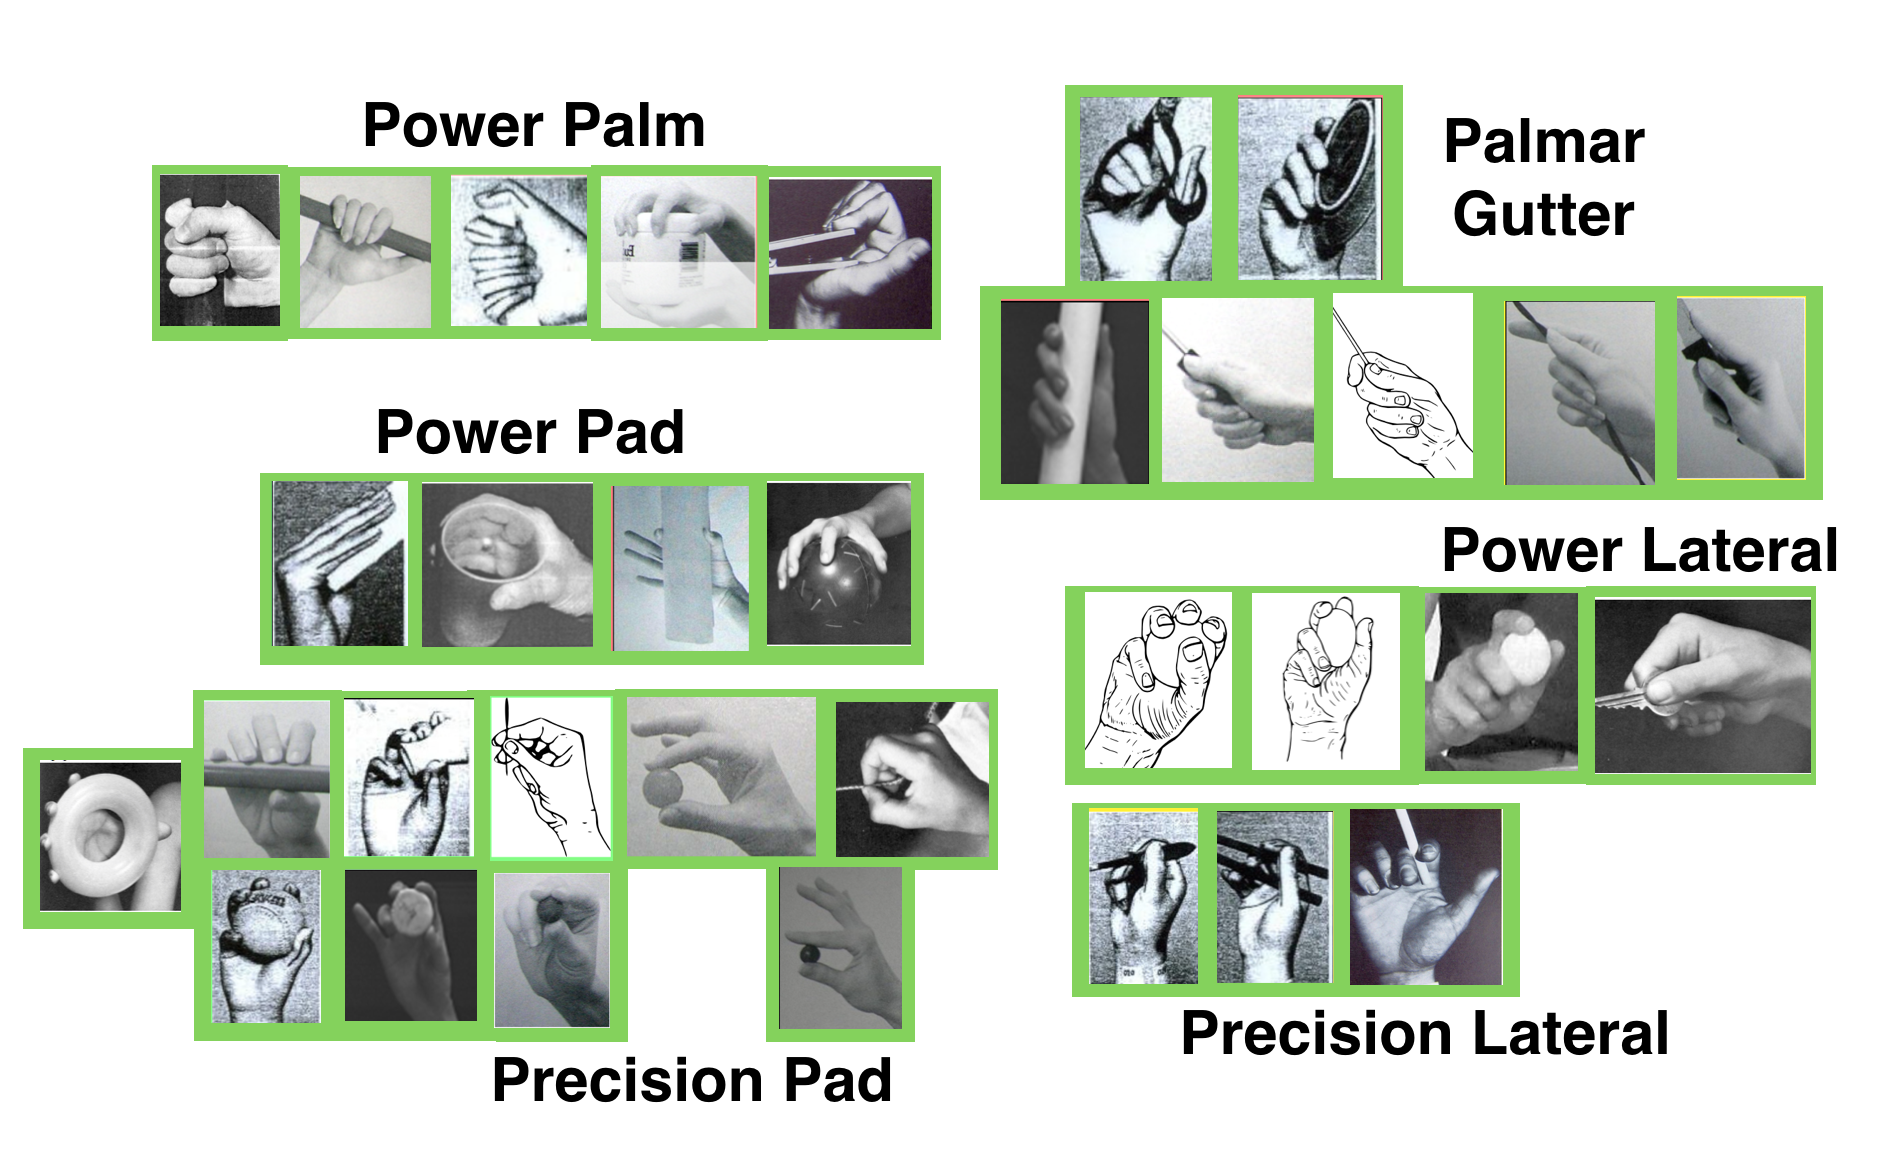
\includegraphics[height=2.2in]{./figs/sixGraspTypes.png}}
{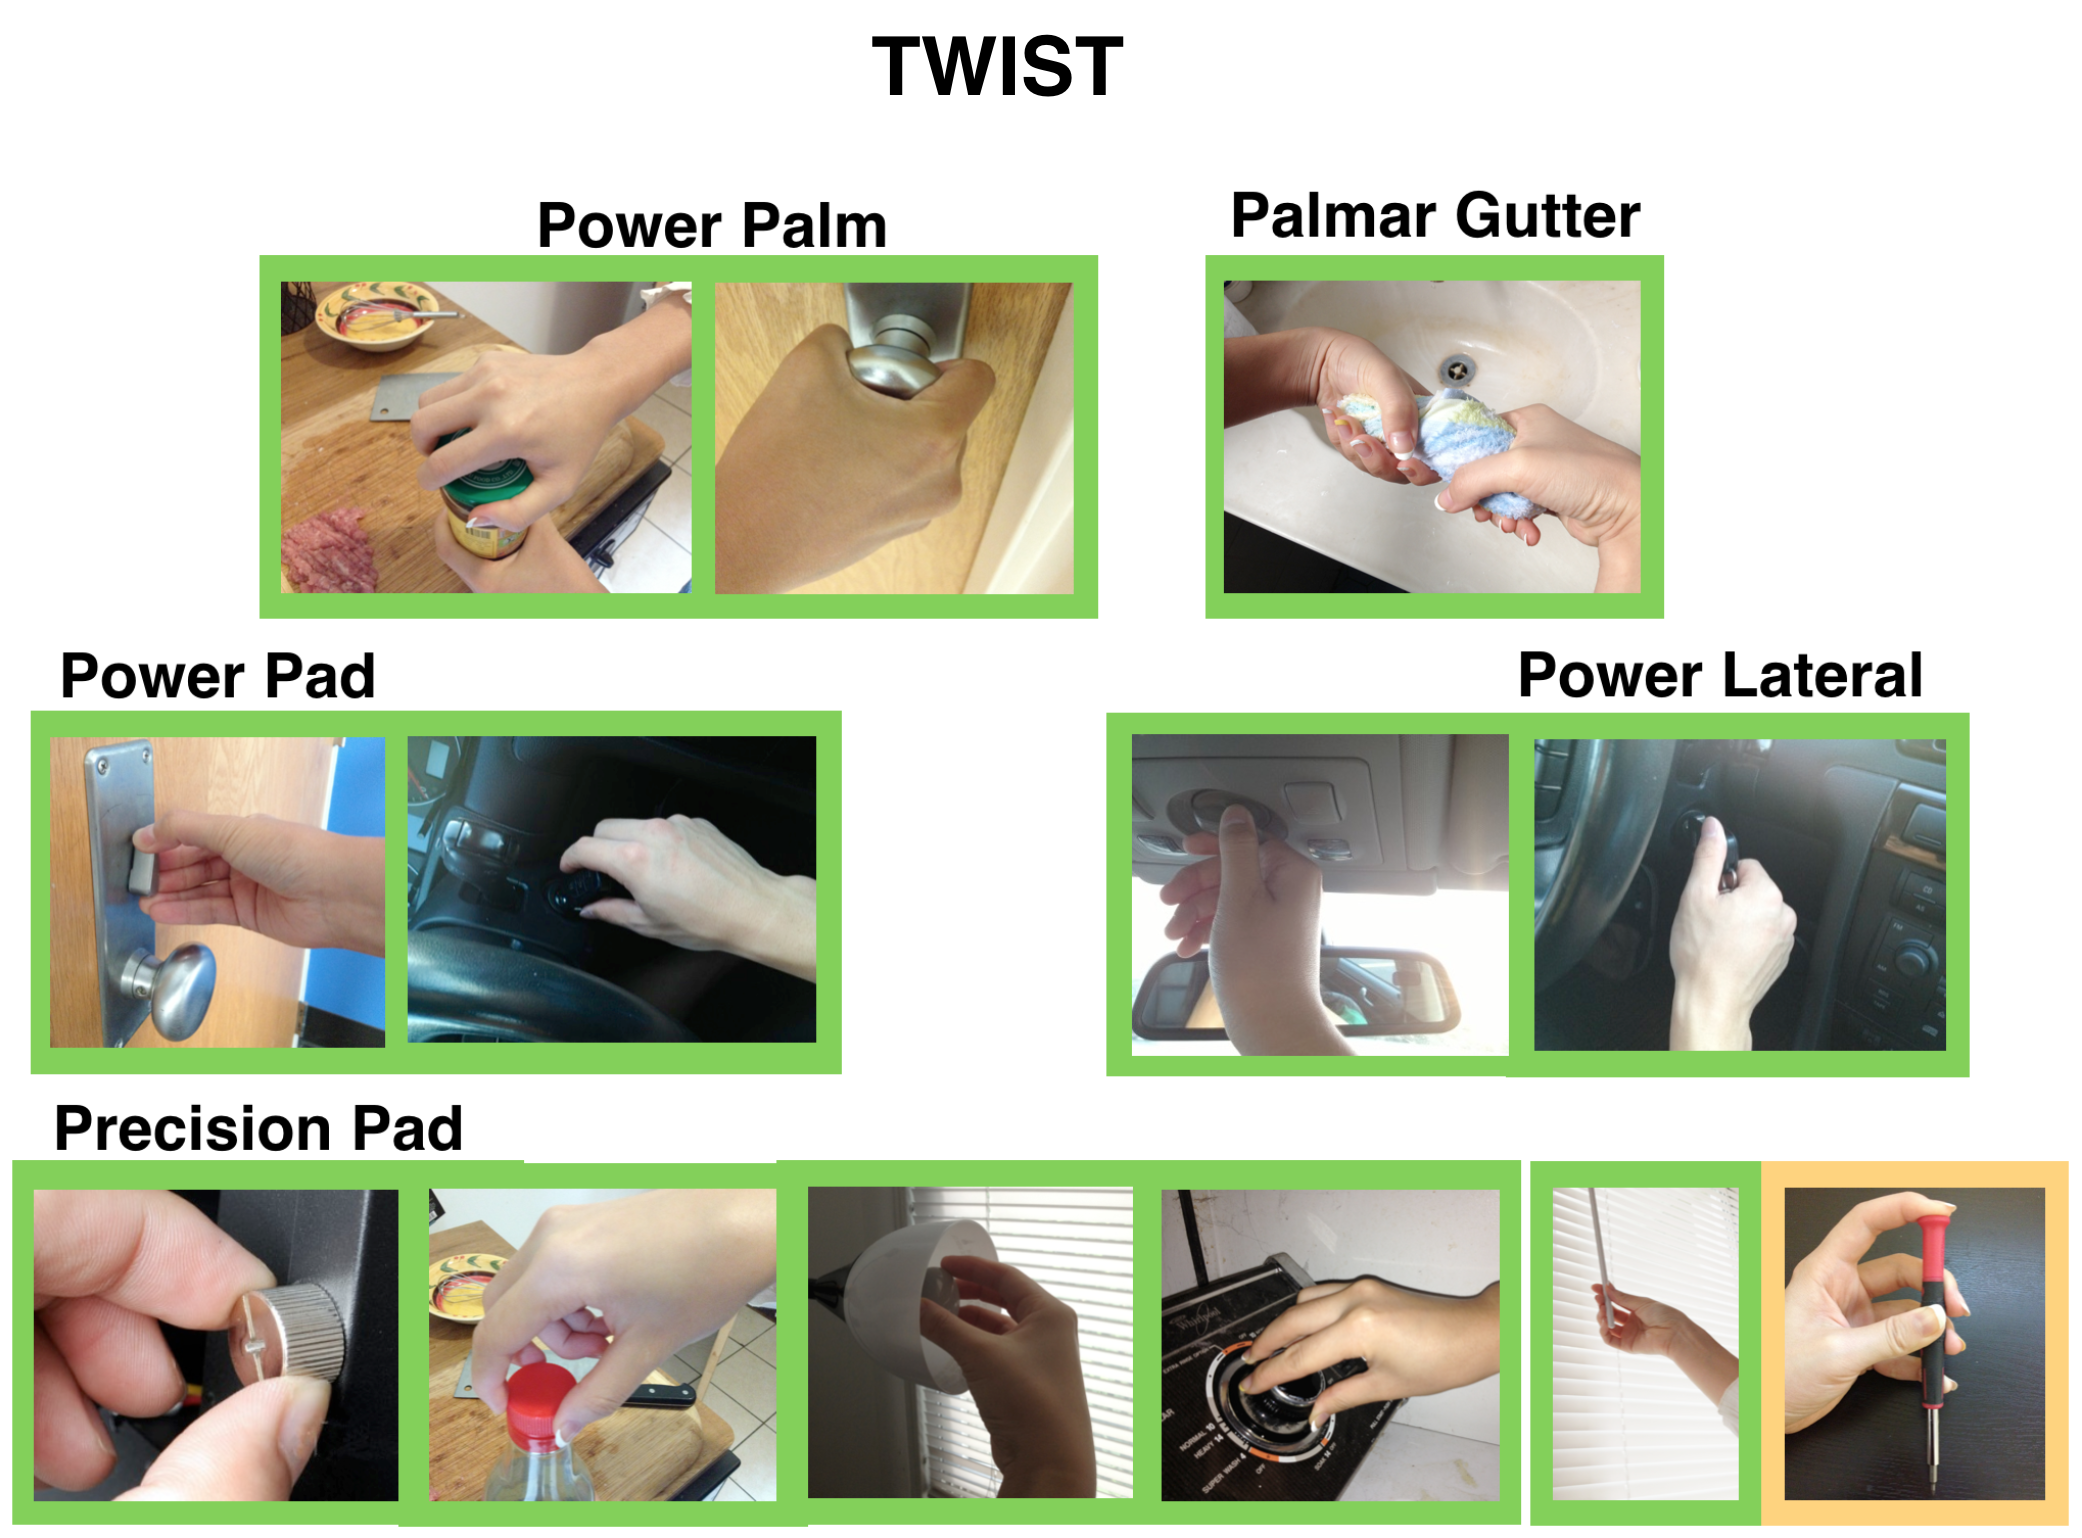
\includegraphics[height=1.8in]{./figs/twistGraspTypes.png}}
%{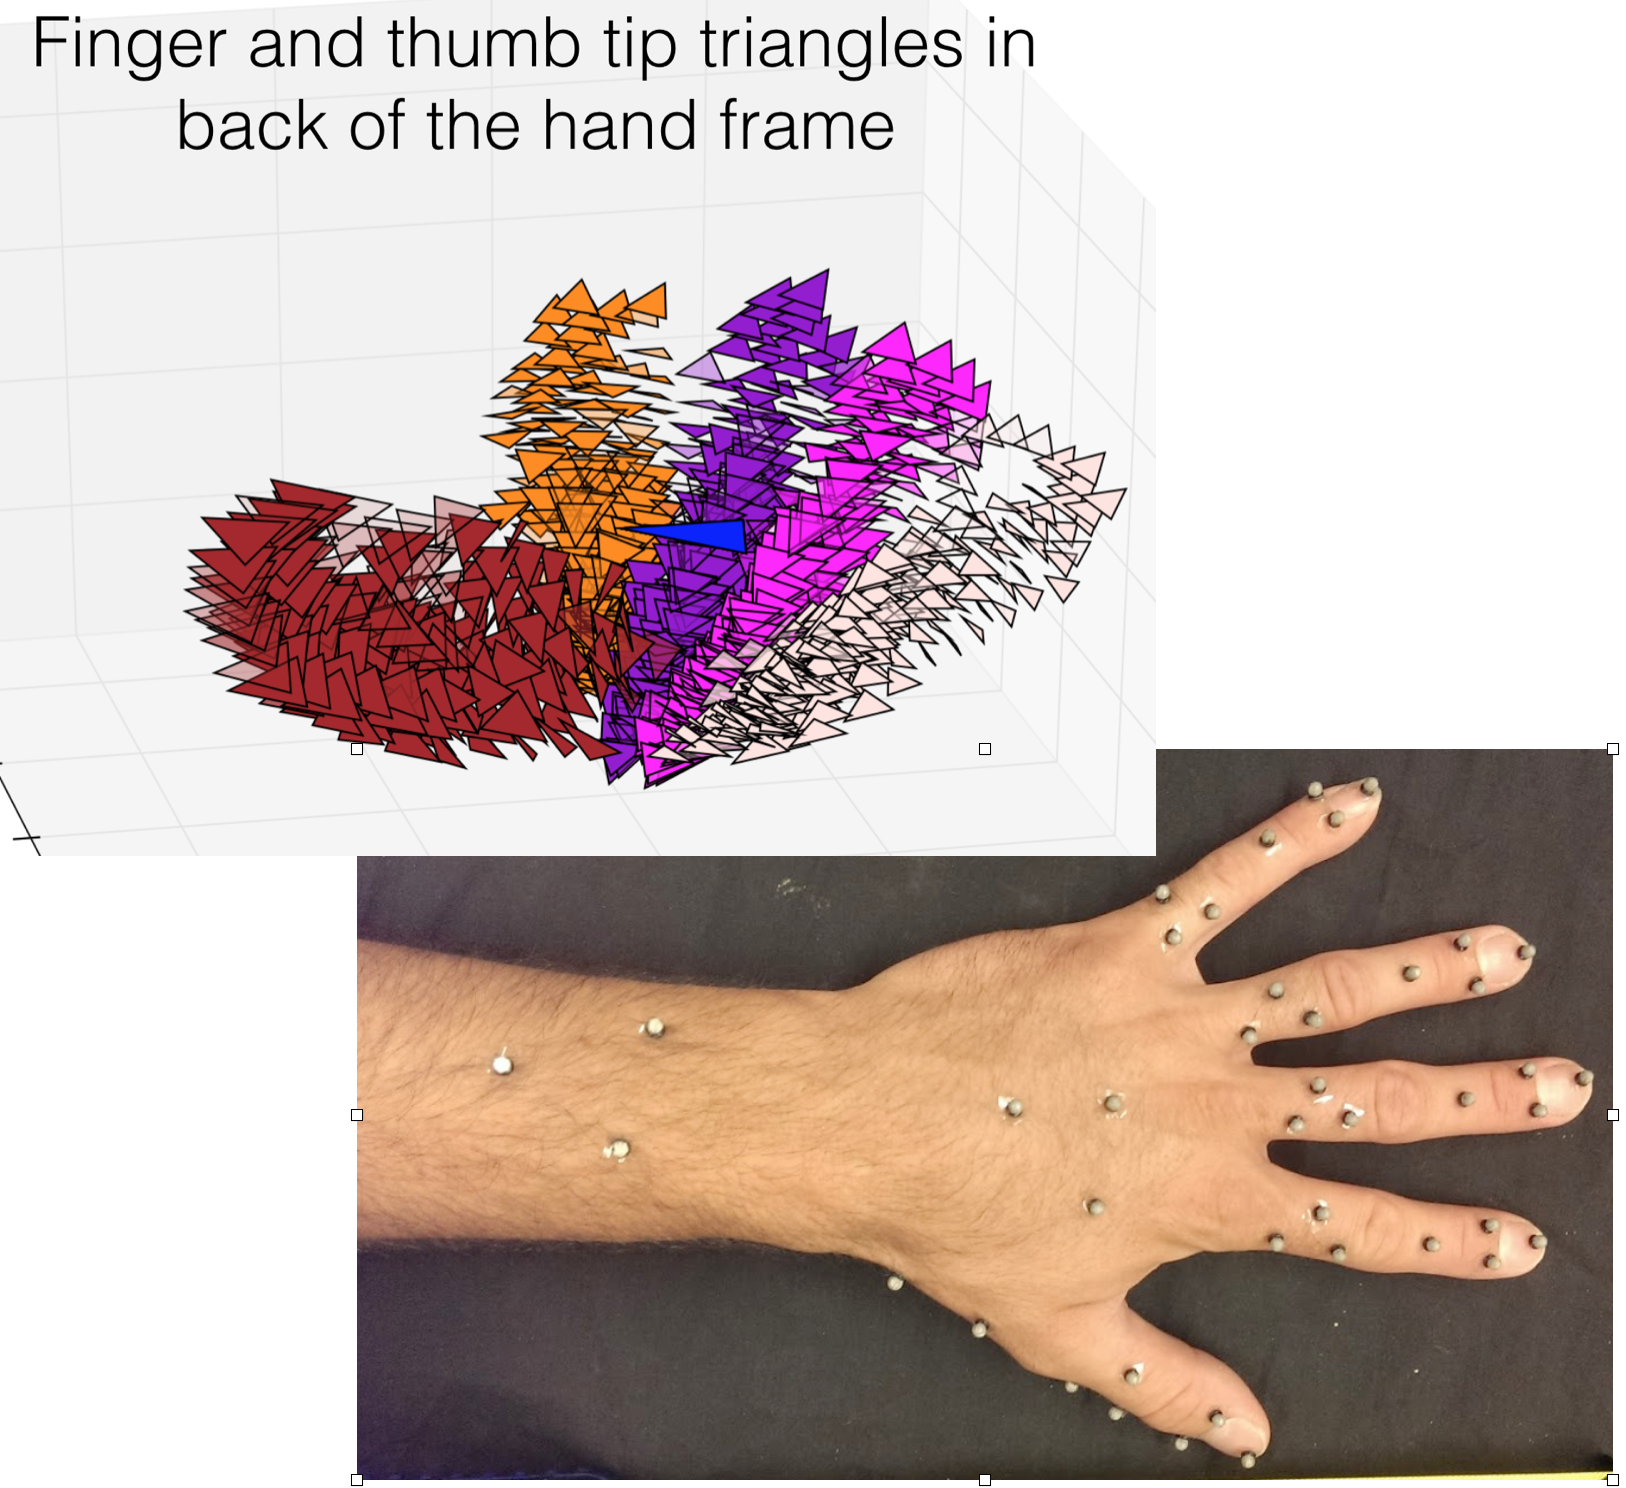
\includegraphics[height=1in]{./figs/mocap.png}}
\end{center}
\vspace*{-0.2in}
\caption[]{(Left) The 33 grasps of the Feix et al. taxonomy \cite{feixgrasp} can be grouped into six classes. (Right) Examples of 5 of these classes in use for the ``twist" action.}
\label{GraspNet}
\end{figure}

To tackle dexterous manipulation head-on, we must consider grasping and manipulation in its full complexity.   We take inspiration from human dexterity.   Full scale humanlike dexterous manipulation may appear enormously complex.   However,  we have observed a relatively small number of grasping tasks and manipulations that are used over and over, with common actions linked to one another, forming what we call Grasp Nets.   These Grasp Nets give us a way to proceed without oversimplifying.  We propose to create Grasp Net benchmarks to cover expanding portions of the dexterous manipulation space.   In tandem, we will develop evaluation procedures that test ability of a mechanism to accomplish Grasp Net tasks in the presence of uncertainty.   One project goal is to create and debug these tests to contribute them to the Roadmap to Progress Measurement Science in Robot Dexterity and Manipulation \cite{falco2014roadmap} where evaluation metrics for dexterous manipulation are needed.   

In this section, we provide some examples to illustrate the idea of a Grasp Net and some of the organizing principles we have observed through various human subject studies \cite{Liu2014, JiaDatabase, Chang:2009:RSSWorkshop, Chang:2014, liu2016annotating}.    These observations are as yet unpublished.

Consider first the grasp taxonomy recently developed by Feix and colleagues \cite{feixgrasp}, which pulls together the wealth of research on grasp classification over the last century.   There are 33 grasps in this taxonomy.  However, we find that they can be placed into six groups (Figure \ref{GraspNet}, Left).  Variations within a group depend mostly on object geometry, and occasionally function (scissors, knife, chopsticks).    Figure \ref{GraspNet}, Right shows examples of the ``Twist" action, uncovered in one of our studies \cite{liu2016annotating}.    Twist actions are found for five of the six categories.   Only the last, Precision Pad, requires intrinsic motions of the fingertips to achieve the twisting action.   In the remaining cases, most of the motion is performed by the wrist and/or arm.

We observe common transitions between the six grasping categories shown in Figure \ref{GraspNet}, such that a brief motion causes a robust transition from one grasp to another.   Figure \ref{DexterousExamples}, Right shows several examples, with the different colored arrows indicating some of the transition paths from one grasp to another.   Beyond  transitions between the six grasping categories, a Grasp Net must contain task related manipulations, such as the twist manipulations shown in Figure \ref{GraspNet} and manipulations to acquire and release an object.   One research challenge will be to map out benchmarks of GraspNet metrics of gradually increasing complexity, but such that each one provides full functionality for a set of tasks (e.g., the robot can get some family of objects into the hand, use them for their intended purpose, and put them back where it found them).

As preliminary work, we have collected detailed human motion data of a Grasp Net containing 21 grasps and more than 25 manipulations and have plans for several more such capture sessions.    Our marker set includes 39 markers on the hand and three on the forearm.    It is processed to a subject specific skeleton \cite{Chang:CoR06,Chang:AoR06,Chang:twoAxis08}.   Object models are available and object motions are tracked to allow estimates of likely contacts.  From these contacts, necessary, sufficient, and plausible families of contact forces can be estimated \cite{Li:graspDB07}.

            % Nancy

\section{Evaluations}

Each unit of research will of course be evaluated as we go.  Two overall evaluations are:

\smallskip\noindent
{\bf Generality. }  If we design for specific task families, will the resulting robot hand be robust and capable enough to generalize beyond the specific given examples?   Because we place such importance on robustness in the design process, we believe the answer will be yes.   We will test generality with leave one out tests and by extent of ability to extrapolate beyond the bounds of the object set given in the Grasp Net.

\smallskip\noindent
{\bf  Comparison to existing robot hands.}    Is it possible for existing robot hands to accomplish all grasps and manipulations within the grasp net?   If not, what fraction can they achieve, based on kinematic structure and load capabilities alone?    We can obtain experimental comparisons of our new hands vs. the Shadow, Barrett, Robotiq, Kinova, and other Hands available to us at CMU.   Our hypothesis is that we will be able to exceed capability and robustness of existing hands in traversing the Grasp Net Benchmark with relatively few actuated degrees of freedom and low cost.   We anticipate that the result may look quite different from the typical dexterous hand existing today.
         % Nancy

\section{Comparison to Related Work}

Design optimization for robot hands has been considered by a number of research groups, and just a few examples are mentioned here.   Salisbury  designed the Stanford/JPL hand to optimize ability to manipulate a small object held in the fingertips \cite{salisbury1982articulated}.  Dollar and his colleagues optimize hands to improve ability to capture the object in a grasp and to maximize workspace while holding a grasped object, and considers the manipulation task of lifting an object from a table with a two actuator hand \cite{borrasDollar2015,ma2014linkage,odhner2015stable}.     Ciocarlie and colleagues optimize a hand to enclose objects as well as possible, whether they be small and flat or larger and round \cite{ciocarlie2014velo}.    Hammond III and colleagues consider which joint ranges of motion can be reduced (or even eliminated) while maintaining ability to achieve a fixed set of grasps \cite{hammond2012towards}.   Bicchi and his colleagues have explored the idea of adaptive synergies in the design of robot hands \cite{catalano2014adaptive}.   Birglen and Gosselin discuss optimization of underactuated hands in part to avoid the phenomenon of ejection \cite{birglen2006geometric}.    We are inspired by these and other efforts in robot hand design optimization and wish to take the next leap to optimize for complex manipulation tasks observed to be critical for dexterity in human environments.

There have been many exciting highly dexterous hands designed, some with the explicit goal of duplicating or exceeding the capabilities of the human hand.   Just a few examples are found in these references \cite{jacobsen1986design,vande2004act,ShadowHand,mouri2002anthropomorphic,lovchik1999robonaut,grebenstein2011dlr,xudesign}.    Perhaps in contrast with some of these works, we begin with the goal to achieve a given network of grasps and manipulation actions, with the approach to make the hand exactly as capable as it needs to be -- not less and perhaps not more -- because adding limits can help.   Our hand may or may not look much like the human hand.   How it comes out will depend on the design elements we provide and what is needed for it to do the required manipulations in a robust manner.

There has been a virtual explosion of ideas on how to use rapid prototyping techniques in robot design \cite{dollar2010highly}, in soft robot design \cite{hirose1978development,deimel2015novel,rus2015design,wehner2014pneumatic,polygerinos2015modeling}, and design of compliant elements such as joints \cite{kuo2016novel}, making this a great time to be exploring the research problems of this proposal.

There has been much work on grasp and manipulation analysis that is also very inspiring \cite{trinkle1990planning,prattichizzo2013motion,prattichizzo1997consistent,lin2000stiffness}.  We especially appreciate the points of view that we can use "defective" mechanisms to our advantage, that local stiffness properties are important for computing quality metrics, and that we wish to configure the mechanism so that abstractly "if we just squeeze," good things will happen.    We expect to build on and extend this research, which will become more and more valuable as we build robots which exploit limits, singularities, asymmetries, and highly coupled action as a matter of course.

The research of Abeel with Levine and colleagues \cite{finn2015deep,kumaroptimal,levine2015learning} suggest that learning manipulations on real robots is possible with small numbers of iterations.   We expect even faster learning and more generality and robustness because the mechanism is designed exactly to do the manipulations is is performing.       % Nancy


\section{Broader Impact}

The expected result of this proposal is robot hands that are robust, inexpensive, dexterous, and as simple as they can be to achieve their function.     The long term promise is dexterous co-robots that can contribute in all corners of life, rendering competent assistance in manual tasks to improve our quality of life, our health, and our safety.    Example application areas include manufacturing, rehabilitation and prosthetics, assembly / disassembly operations in space, and personal robots that are able to assist with shopping, cooking, maintenance, dressing, and feeding, allowing elderly or disabled individuals the dignity to live longer in their own homes.

\paragraph{International Collaboration.}
We are have active collaborations with ETH Zurich, we host students from the University of Karlsruhe in Germany, and we anticipate productive collaborations with Paul Kry's group at McGill University in Canada in connection with the proposed research (see letter).    

 \paragraph{Graduate education.} This project will have a significant impact on graduate students.   Students will be encouraged to work on the project directly, and to experience the research through course offerings at CMU, including 
 15869 Computational Aspects of Fabrication and 16899 Hands: Design and Control for Dexterous Manipulation.  

 \paragraph{Undergraduate education.}   We expect numerous undergraduates to be involved in this research as well.    PI Pollard has advised more than 20 undergraduates, more than one third female, most involved in NSF supported research, and many who have gone on to graduate school.    Both PIs offer advanced undergraduate courses that will expose undergraduates to the proposed research and encourage them to get involved themselves.

 \paragraph{Participation of underrepresented groups.}  Pollard has mentored four women through the CRA-W Distributed Research Experiences for Undergraduates (DREU) program, and has advised 7 female graduate students and 8 female undergraduates, three of whom have gone on to PhD studies at Stanford and CMU.

 \paragraph{Public and K-12 outreach}
Pollard has been involved in discussing robotics and 3D printing of functional objects at local elementary schools to increase interest in STEM and Maker topics, especially with young girls.  The proposed research offers a great opportunity for K-12 outreach, due to the hands-on nature of the robot hand prototypes which will be generated at many stages of the research project.   We will introduce young students to these prototypes and to robotics in general, both through annual CMU outreach programs and through our own school visits and talks.

 \paragraph{Dissemination.} 
 Dissemination will be primarily through publication in conferences and journals and participation in and organization or relevant workshops.    Prototype designs will be made available in the form of design files and instructions to speed progress in this critical area.   Human manipulation data collected as part of this project will also be made available online.

    % Nancy

\section{Results from Prior NSF Support}

PI Pollard brings decades of experience in grasping and manipulation analysis and experience working with various robotic hands and systems.   PI Coros brings experience in optimal design of creative, complex mechanisms to accomplish user specified tasks, as well as 10 years of experience in control algorithms for complex tasks.     This combination of skills is critical for designing and creating robot hands with the capability and skills to grasp and manipulate robustly in complex, real-world scenarios where humans and robots live and work together.

\begin{figure}
\begin{center}
{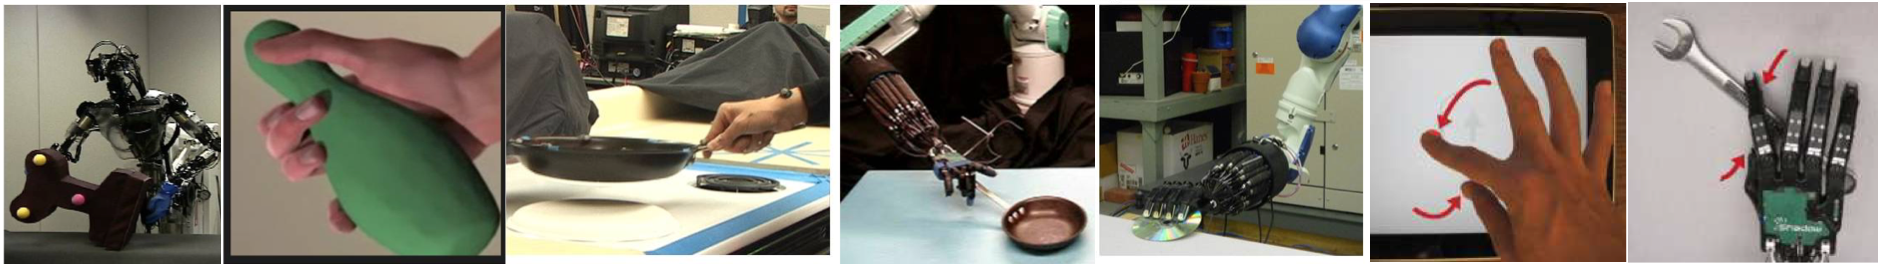
\includegraphics[width=\linewidth]{./figs/nspPrior}}
\end{center}
\vspace*{-0.2in}
\caption{\small Examples show prior research of PI Pollard in transfer of grasp and manipulation tasks, grasp planning with preparatory manipulation, and teleManipulation.}
\label{fig:nspPrior}
\end{figure}

\paragraph{Pollard's prior work on physics-based grasping and manipulation.} 
PI Pollard has extensive experience in grasp and manipulation planning, transfer, and optimization (Figure \ref{fig:nspPrior}).   She has developed algorithms for grasping and manipulation that allow fast transfer of examples from human to robot and generalization to varying object geometries in a manner that is both fast and provides bounds on performance \cite{pollard2004closure,Pollard:WAFR02,pollard2005physically,Li:graspDB07}.   She and her students have performed numerous human subjects studies to better understand the complex process of grasping in real-world situations \cite{Chang:2009,Chang:JMB10,illing2014changing,liu2016annotating} and followed up with more highly capable robot planning algorithms and quality metrics that function well for robot grasping in the presence of uncertainties \cite{Chang:ICRA10,Kappler:2012,kim2013physically}.   She has studied human-in-the-loop manipulation (teleManipulation) \cite{Toh:2012,chung2015quadratic,Kim:CGA11} and examined anatomical considerations of the human hand that may lead to better robot hand designs \cite{pollard2002tendon,fu2006importance,Chang:twoAxis08,Chang:CoR06,Chang:AoR06}.


\paragraph{Results from Prior NSF Support.}
Pollard has been funded by NSF awards \emph{CCF: Capturing and Animating the Human Hand: Robust Recovery of Hand-Object Interactions} NSF CCF0702443 (PI:  Pollard  6/07 - 5/11, \$325,000)  and \emph{CGV: Small: Simulation Motion Capture of Dexterous Manipulation} NSF IIS1218182 (PI:  Pollard  8/12 - 7/16, \$499,838).
{\bf Intellectual Merit:}  Results include taxonomies of everyday grasps, manipulations, and manipulation actions prior to grasping, findings on rotation prior to grasping, a novel algorithm for planning robotic tasks with preparatory manipulation, quality metrics for grasping that reflect real-world uncertainties and physics, robust
algorithms for capturing human hand skeletal structure, fast algorithms for simulation of deformable systems, a novel interactive system for guiding
simulations, a system for robot teleManipulation using multitouch, and an investigation of new
representations for motion that are meaningful across 
individuals and species (including robots).  This award resulted in the following
publications
\cite{liu2016annotating,chung2015quadratic,Liu2014,illing2014changing,kim2013physically,Toh:2012,Chang:2014,Gatesy:2011,Kappler:2012,Kim:ToG11,Kim:CGA11,Koonjul:ICRA11,Chang:JMB10,Chang:ICRA10,Kappler:Humanoids10,Chang:2009,Chang:twoAxis08,Chang:Humanoids08}.
{\bf Broader Impact:}  In addition to top venues in Robotics and Computer Graphics, results
have been published in the Journal of Motor Behavior, the Journal of
Biomechanics, the Journal of Theoretical Biology, and
in the book ``The Human Hand: A Source of Inspiration for
Robotic Hands.''  These grants supported two female PhD students, Lillian Chang and Yuzuko Nakamura,
whose dissertations contained many of the core research findings.  They also provided partial support for four masters students (two female), three undergraduates (two female),
and one postdoc.

\begin{figure}
\begin{center}
{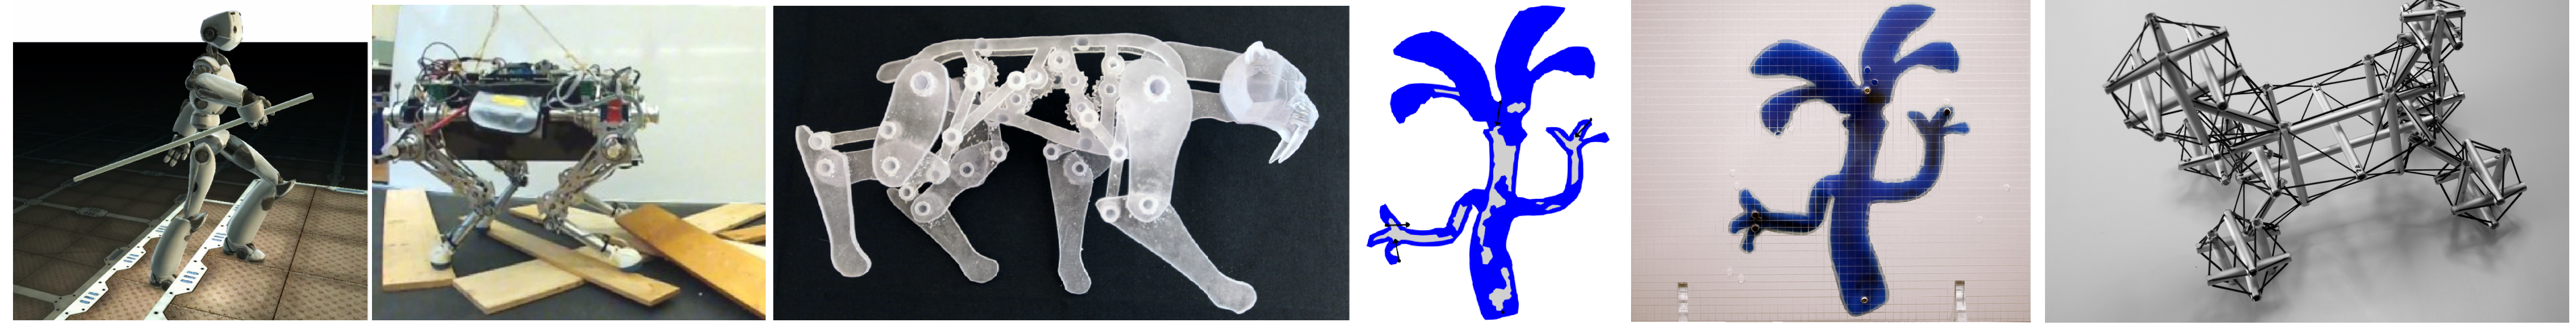
\includegraphics[width=\linewidth]{./figs/corosPrior}}
\end{center}
\vspace*{-0.2in}
\caption{\small Examples show prior research conducted by PI Coros in control methods for locomotion and manipulation, computational design of complex mechanical structures and digital fabrication.}
\label{fig:corosPrior}
\end{figure}

\paragraph{Coros's prior work on computational design and digital fabrication.} PI Coros has extensive experience in computer animation, robotics, computational design and digital fabrication, which are all areas of crucial importance for this proposal. Within the field of computer animation, the PI has developed physics-based methods that enable virtual actors to move autonomously using the same principles that underlie human and animal motions \cite{Yin08,Coros08,Coros09,Coros2010,Coros2011}. The PI extended these motor control models to apply them to \emph{StarlETH}, a dog-sized quadrupedal robot \cite{Gehring2015,Gehring2014,Gehring2013}. In addition to this line of work, the PI is investigating mathematical models and computational approaches to significantly simplify challenging design tasks that traditionally require a great deal of domain-specific knowledge. For example, he has developed several computational design systems that allow casual users to quickly design 3D printable mechanical automata \cite{Coros2013,Thomaszewski14CDL,Megaro14Chacra,Bacher2015}. Such complex mechanical assemblies combine geometric features, functionality and motion through a complex set of kinematic relationships and are notoriously difficult to design with traditional approaches. The PI's research has also ventured into the domain of multi-material 3D printing. For example, the goal of one of his recent projects was to automatically determine the distribution of rigid and soft materials within 3D printed objects such that the way in which they deform under the influence of external forces can be controlled \cite{Skouras2013}. This work complements other research efforts aimed at controlling the elastic properties of fabricated objects \cite{Gauge2014,Jesus2015} and builds on the soft body simulation models investigated by Coros and his colleagues \cite{Coros2012,Hahn2012,Schumacher2012}. Building on this body of work, this proposal will enable the design of a new class of robotic hands that are specifically designed for dexterous manipulation tasks.

\paragraph{Results from Prior NSF Support.} PI Coros is an NSF beginning investigator with no prior support.

   % Nancy




%\section{Timeline}    % Nancy

%\input{punchlist.tex}   % ALL!

%\section{Misc Notes}


BENEFITS OF JOINT LIMITS AND INTRINSIC COMPLIANCE

We can simulate joint limits in software, so it is an obvious question why build them in?

Combat uncertainty.   If you push yourself against a joint limit, you know where you are in that dimension.

Reduce complexity (fewer motors .. it may only be necessary to actuate in one direction and use compliance to passively drive a mechanism back to its limit)

Reduce power (smaller motors .. the joint limit can resist arbitrary forces by passing them up to the much stronger arm and torso of the robot  ..  ideally all the way through to the ground .. passive forces can reduce the required operating range for the motors)

Reduce sensor requirements (fewer and perhaps simpler sensors .. multiple joints may not need to be so carefully coordinated with one another)

Perform actions more robustly (e.g., if one finger is pushing into a joint limit "corner", there may be a robust region within which an appropriate opposition force may be created)

The simple example can illustrate all these things...




Finger surface characteristics
How do you compose multiple systems that are all one DoF?
  clutch or ratchet mechanism

Relative configurations of contacts matter more than the absolute coordinates

Maximum tendon approach .. align tendons with known forces
Force families describe family of forces that is sufficient

Does Yong-Lae have a student who is trying to wrap sensors around objects? -- Nancy
Ask Scott Hudson? -- Stelian

Previous work -- design a linkage to achieve a given end effector motion .. or fit multiple points
if not enough flexibility, back off 

Tendons, linkages, soft fingers

digital fabrication
   understand the space of designs that are achievable .. variable compliance across a structure
   incorporate this knowledge in the design process
   print some compliant "fingers" with different compliance properties -- Stelian

new tools for analysis of grasping and manipulation with compliance and joint limits
new tools for design of mechanisms with same 



WHAT DO WE MEAN  BY DEXTERITY IN THIS DOCUMENT?

Here is from the NIST roadmap:
"The term ?dexterity? itself must be fully and formally defined, along with its constituent functional capabilities. Examples of functional capabilities range from simple tactile sensing (contact achieved or not) to force-guided insertion of parts for snap-fit assemblies. "

One part of dexterity involves reconfiguring the object within the hand in a robust manner [page of examples?].    We focus on this aspect, including picking the object up and replacing it, with intent to make the mechanical design itself as supportive of such motions as possible.

There are other aspects of dexterity that are not covered (e.g., force-guided assembly).

This can be done as a second part of the project .. we would want something like a general purpose device in the manner of the RCC where the mechanism does as much as possible to achieve assembly operations in situations with error as passively as possible.

We could also look at what sensors can be most effective in improving the robustness of grasps and manipulations in our grasp net.


Point 1.  We observe that there are a few specific dexterous motions that are extremely useful.  These motions allow us to acquire objects, move between grasps, and to accomplish tasks such as twisting (e.g., a doorknob) or pressing (e.g., the trigger on a spray bottle).    We tackle the problem of robot hand design in a way that makes these dexterous motions central.

Point 2.  We illustrate that carefully placed joint limits and compliance can be of extreme benefit for design of a robust and efficient manipulator capable of dexterous manipulation.    Everyone should be designing with these elements in mind.

Point 3.   We provide tools for design and analysis that focus on dexterous manipulation, built-in compliance, and joint limits

Point 4.   To improve opportunities for success of a dexterous manipulation action, we introduce a technique for self assessment of a starting point leading into a dexterous manipulation.


Expected contributions include:
	(1) Develop / identify the grasp web, which consists of specific grasps or grasp families and nodes, along with the following links:
		> acquire grasp
		> transition between grasps
		> adjust grasp
		> use a tool, perform an action
		> release grasp
	(2) highlight joint limits, rest configuration, and intrinsic stiffness as critical design components for robust manipulation 
	(3) develop design and analysis tools to accomplish a given grasp web:
		> select mechanism degrees of freedom
		> place joint limits
		> route tendons (or otherwise customize delivery of force from actuators)
		> assign rest configuration 
		> assign intrinsic stiffness
	(4) develop a self assessment test and accompanying adjustments that set the  grasp up for a probabilistically more successful manipulation
		> I don't remember what this is
	
The grasp web (1) defines a set of relative postures, motions, and forces between contacts (e.g. finger pads) that must be achieved.

The analysis tools (3) provide us with a principled way to write down characteristics of acceptable solutions and search this space for robot hand designs that are dexterous, yet have few degrees of freedom and are efficient and robust.



ADD SELF ASSESSMENT OF GRASPS THROUGH FORCE TESTS

Postulate that achieving some grasp is pretty easy but adjusting it for efficiency or for a successful manipulation is harder

Technical:

(A) Why I believe there is a grasp net:
	> extensive investigation of human grasping and manipulation in the wild
	> at first there seem a bewildering variety of grasps
	> but many are similar, and we have canonical ways of shifting into, out of, and between them
	> show a sample
	> explain what's left to do
	
(B) Show benefit of joint limits
	> simpler mechanism
	> stable strategies for ensuring you are in the right place
	> more robust to errors (show with an example?)
	
	INCLUDE FORCE SENSITIVE JOINT LIMITS (E.G., A NOTCH)

(C) Design with joint limits

(D) Manipulations to improve the grasp
	> self assessment
	> correction


SHOULD DISCUSS SOMEWHERE CONTRIBUTIONS TO PLANNING OF THE GRASP NET

SHOULD DISCUSS SOMEWHERE HOW INTERACTIONS WITH THE ENVIRONMENT ARE INCLUDED (E.G., COMPLIANTLY GET THE FINGERS IN AROUND OBJECTS)

MENTION USE OF THE YALE BENCHMARK SET FOR EVALUATION
	CODIFY MANIPULATIONS OF OBJECTS IN THIS SET?
	HOW DOES THIS LINE OF THINKING INTERACT WITH TARGETING PERFORMANCE TESTS LIKE SHAP?
	
MAYBE WE HAVE TO ADDRESS THIS POINT:
Quote from the Robotics Roadmap:
Progress in robotic grasping and manipulation very likely will go hand in hand with the development of novel hand mechanisms. At the same time, participants felt that the potential of current hand technology was not fully leveraged by existing grasping and manipulation algorithms. It is therefore conceivable that many interesting and relevant applications can be addressed with available grasping and manipulation hardware.	



"The NIST
workshop identified the need for benchmarking dexterity, similar to the Southampton Hand 
Assessment Procedure (SHAP) that was developed as a means to measure the performance of upper limb 
prostheses [5].  SHAP defines 26 tasks using 8 abstract objects and
14 activities to be performed by a subject 
fitted with a prosthetic device.  Measurements of success and speed are used to calculate overall performance of 
prostheses.  The procedures discriminate between functional and force limitations. "


BACKGROUND

There are quite a lot of good general ways to evaluate a hand, and any of these evaluation criteria can form the basis for design optimization
	- specific grasps (Brock uses Feix et al.)
	- manipulability (Salisbury and others)
	- grip strength, sensing capabilities, etc.   (NIST report)
	- Southampton Hand Assessment Procedure
	- many others .. see the published review of hand dexterity assessments
		> Minnesota Manual Dexterity Test
		> Jebsen Test of Hand Function
		> Functional Capacity Evaluation with Matheson Panel System
		> Purdue Pegboard
		> O'Connor Dexterity Test
		> Bennet Hand Tool Dexterity Test
	
We also like the specific grasps technique, but we have to look at the complete picture (the grasp web)



From the Robotics Roadmap / Space exploration
Manipulation is defined as making an intentional change in the environment. Positioning sensors, han- dling objects, digging, assembling, grappling, berthing, deploying, sampling, bending, and even posi- tioning the crew on the end of long arms are tasks considered to be forms of manipulation. Arms, cables, fingers, scoops, and combinations of multiple limbs are embodiments of manipulators. Here we look ahead to missions? requirements and chart the evolution of these capabilities that will be needed for space missions. Metrics for measuring progress in manipulation technology include strength, reach, mass, power, resolution, minimum force/position, and number of interfaces handled.


Concrete examples of fine manipulation.
	- some can come from Elliott and Connelly

Existing manipulators -- why are these things hard?

	- consider roll, twiddle, pinch
		- we need a justification of why use the Elliott and Connelly motions as a starting point
			- see comments on the paper below

	- we can analyze workspace
		- however, even if we find the workspace to be adequate, it is still difficult to control those motions
		
	- suppose we consider the maxims that:
		- passive is better than active in achieving a motion
		- compliance is better than non-backdrivability
		- using rigid components to push forces/torques proximally to stronger joints is always a good idea
		
	- necessary improvements are:
		- carefully designed joint limits
			- can we develop a theory of where to put stiffness and where to put compliance and use it in design?
				- overall rest pose for "averaged out" assistance with support
				- joint limits at workspace boundaries wherever possible and with priority where large forces are supported BUT no work must be done
				- compliance where the hand must adapt to object shape and collisions (many examples in Jia video)
		- careful design of passive stiffness
		- careful placement of actuations
		
	- joint limits are usually seen as something to avoid (Google scholar search results)
		- however, robot hands often may exploit locking mechanisms or lack of backdrivability 
			- Krut et al. (mentioned below) discusses this less discussed point
			- if joints are not backdrivable, they can always act as though they are at a joint limit
			- however, all interactions will be stiff
		- backdrivable joints give compliance, but must be carefully controlled to give support
		
	- quotes from "Stable, open-loop precision manipulation with underactuated hands"	
		- "reduction of the number of actuators and constraints can make within-hand manipulation easier to implement and control"
		- "under actuated, passively adaptive grippers can also be tuned to make in-hand manipulation possible with minimal sensing"
		- "we will see that the ability to grasp without locking the fingers is a key to achieving robust in-hand manipulation"
		- useful analysis of the effects of actuator motion on a grasped object
		- "if the stiffness of a contact constraint is large relative to the constraint's magnitude, then it is quite possible for a small perturbation of the actuators to cause the fingertip to lose contact, or to crush the object"
		
	- Falco et al. article pending IEEE publication
		- "This document presents the beginnings of a framework for robotic hand performance benchmarking. Many of the concepts presented are the results of an informal working group1 organized by the National Institute of Standards and Technology (NIST) that continues as part of the recently formed IEEE Robotics and Automation Society (RAS) Robotic Hand Grasping and Manipulation (RHGM) Technical Committee2. "
		- reference this in the context of evaluation
			- example, if planning a series of hurdles that a design must be capable of achieving .. would those become benchmarks?
		- functional tests, to evaluate purposeful grasping and manipulation actions were not included in this document
		
	- Elliott and Connelly
		- state a belief that intrinsic manipulation movements "can be reduced to three basic classes, which we call simple synergies, reciprocal synergies and sequential patterns"
		- "Most kinds of intrinsic movement involve a single co-ordinated pattern of digit movements. "
		- "However, some other patterns entail the independent co-ordination of digits in a characteristic sequence"
		- "Within the simultaneous patterns, simple and reciprocal synergies are distinguished. Simple synergies are de- fined as those in which all movements of the participating digits, including the thumb, are convergent flexor synergies. There may be an alternation of flexor and extensor synergies, as in repeatedly squeezing a rubber bulb, but in either case the movements of all the digits are the same. Reciprocal synergies, by contrast, involve combinations of movements in which the thumb and the other participating digits show dissimilar or reciprocating movements, such as flexion of the fingers with adduction or extension of the thumb. The justification for distinguishing these two classes of synergy is that only in the case of reciprocal synergies is the thumb's capacity for movement independent of the fingers used in the manipulation of objects. A high proportion of intrinsic movements appear to fall into this category."
		- the authors observe that even in writing (dynamic tripod), the three radial fingers move in a flexor/extensor synergy, creating vertical elongation of the letters
		- "We have the strong impression that use of the radial aspect of the index in twiddle confers a greater potential power to the movement, and also a more stable hold upon the object before or after movement. It is possible to demonstrate a shift to a more radial use by requiring a subject to tighten progressively stiffer nuts."
		
		
	- Krut et al. Extension of the Form Closure Property to Underactuated Hands
		- deals with condition where contacts may not be fixed in space
		- check that some unidirectional kinematic constraint operates in any direction the object may care to move
				
	- Prattichizzo et al. OnTheManipulability.pdf for categorizing manipulability of underactuated hands
		- there are a number of references relating to synergies here .. where do the synergies come from?    PCA in all cases???
			- synergies in robot hand design [3]
			- impedance controller derivation including synergies implemented on DLR hand [5]
			- mapping between human and robot synergies with different kinematics [6]
			- control of force and motion of grasped object using synergies [7]
			- synergies and grasp quality [8]
			
	- how do you design where to use limits and where to have compliance?
		
	- one interesting thing is the interaction between degrees of freedom in thinking of joint limits
		- index finger is a good example, with available motion decreasing as the finger is flexed
		
	- what about the idea of simplicity in design
		- more DoF at joint limits is simpler (easier to achieve with confidence and limited sensing)
		- tendons aligned with a desired direction of motion is simpler
		
	- a high level of compliance is desirable to avoid damaging objects and to simplify execution of everyday behaviors
		- we can find a lot of high compliance actions in the Jia and Daniel video
		
	- compare controls for shadow hand to an idealized situation with:
		- flat plane (joint limit)
			- eliminates a source of error in reaching and sensing your position
		- single control (e.g., flexor)
			- eliminates a source of error in coordinating your motion
		- passive force aiding the motion (e.g., passive force pressing thumb to index finger for roll or twiddle)
			- reduces errors that can arise in controlling forces
			
		- how do we compare?
			- we can push simple error models through the two scenarios...
		
	
   %  nsp scratchpad .. won't be included

	

%\newpage

%
\section*{Human Subjects Protection}

Data associated with human subjects includes high speed videos, motion capture data, and other data
    modalities collected for everyday manipulation tasks.  As part of
  our study of manipulation, we will collect video and RGB-D data of
  our human subjects in natural settings, and motion capture data,
  force data, and other data modalities in our motion capture lab.




\subsection*{Potential Risks to Human Subjects}

The risks and discomfort associated with participation in these
studies will be no greater than those ordinarily encountered in daily
life or during the performance of routine physical or psychological
examinations or tests.  Should optical markers be used to measure
motion, subjects may experience a small amount of discomfort when the
optical markers are removed (equivalent to removing a bandaid from the
skin.)

\subsection*{Plans for Recruitment}


Subjects will be recruited throughout the CMU campus through posted
advertisements and an email mailing list.   Subjects of both genders
will be recruited equally.  The experiments will be restricted to
adult subjects who give voluntary consent to participate and who will
be instructed that they may terminate their participation in the study
at any time.   A small monetary compensation may be
provided for participation in the study.


\subsection*{Informed Consent}

Subjects will be given a written document outlining the goals of the
study, its duration, and the nature of the tasks they will be asked to
perform.  The consent document will have information on whom to
contact should they have any questions or concerns after the study,
and they will be given a copy of this document to take with them.

The confidentiality statement given to human subjects for our studies
is expected to be worded as follows:

``By participating in the study, you understand and agree that
Carnegie Mellon may be required to disclose your consent form, data
and other personally identifiable information as required by law,
regulation, subpoena or court order. Otherwise, your confidentiality
will be maintained in the following manner: 

Your data and consent form will be kept separate. Your consent form
will be stored in a locked location on Carnegie Mellon property and
will not be disclosed to third parties. By participating, you
understand and agree that the data and information gathered during
this study may be used by Carnegie Mellon and published and/or
disclosed by Carnegie Mellon to others outside of Carnegie
Mellon. However, your name, address, contact information and other
direct personal identifiers in your consent form will not be mentioned
in any such publication or dissemination of the research data and/or
results by Carnegie Mellon.

I understand that the following procedures will be used to maintain my
anonymity in analysis and publication/presentation of any results: (1)
Each participant will be assigned a number, names will not be
recorded. (2) The researchers will save the data file and/or any video
or audio recordings by participant number, not by name. The data and
video will be stored on the web and free access will be granted to
researchers and others. The videotape may be of sufficient quality for
someone to recognize me. I may request to see my data visualized and
may request that particular trials from a session be deleted if I
prefer that my performance not be included in the database. I may
request that the researchers remove the video clips from the web
database at any time in the future.''

\subsection*{Inclusion of Women, Minorities, and Children}

Women and minorities will be recruited equally among all other abled
adult members of the population.   Participants in the study will be
required to be 18 years of age or older.
  % Nancy

\newpage

\bibliographystyle{plain}
\bibliography{./main}

%
%
 \end{document}
 
